\documentclass[a4paper,12pt,3p]{report}
\usepackage{graphicx}
\usepackage[font=normalsize]{caption}
\usepackage{subcaption}
\usepackage{float}
\usepackage{wrapfig}
\usepackage{amssymb}
\usepackage{amsmath}
\usepackage{amstext}
\usepackage[linesnumbered,ruled]{algorithm2e}
\usepackage{multicol}
\usepackage{multirow}
\usepackage[export]{adjustbox}

\usepackage[bookmarks=false]{hyperref}
\hypersetup{colorlinks,
	linkcolor=blue,
	citecolor=blue,
	urlcolor=blue}
	
\usepackage{titlesec}
\setcounter{secnumdepth}{4}

%\usepackage{csquotes}
%\usepackage[style=verbose-ibid,backend=bibtex]{biblatex}
%\bibliography{reference}

%\titleformat{\paragraph}
%{\normalfont\normalsize\bfseries}{\theparagraph}{1em}{}
%\titleformat{\section}[hang]{\bfseries}{Item \thesection:\ }{0pt}{}


\titlespacing*{\paragraph}{0pt}{1.5ex plus 1ex minus .2ex}{1.5ex plus .2ex}
\graphicspath{ {./images/} }
\usepackage[X2,T1]{fontenc}
\usepackage[utf8]{vietnam}
\usepackage{tabu}

\usepackage{fancyhdr}
\pagestyle{fancy}
\fancyhf{}
\fancyhead[LE,RO]{Overleaf}
\fancyhead[RE,LO]{Guides and tutorials}
\fancyfoot[CE,CO]{\chaptername}
\fancyfoot[LE,RO]{\thepage}
 

\DeclareTextSymbolDefault{\CYREPS}{X2}
\DeclareTextSymbolDefault{\cyreps}{X2}

\DeclareUnicodeCharacter{0190}{\CYREPS}
\DeclareUnicodeCharacter{025B}{\cyreps}
\usepackage[left=3.5cm,right=2cm,top=2cm,bottom=2cm]{geometry}
\usepackage{indentfirst}
\usepackage{color, colortbl}
\definecolor{Gray}{gray}{0.9}

\usepackage{tikz}
\usetikzlibrary{calc}

\usepackage{graphicx}
\usepackage{verbatim}
\usepackage{latexsym}
\usepackage{mathchars}
\usepackage{setspace}
\usepackage{footnote}


\setlength{\parskip}{\medskipamount}  % a little space before a \par
\setlength{\parindent}{0pt}	      % don't indent first lines of paragraphs
%UHEAD.STY  If this is included after \documentstyle{report}, it adds
% an underlined heading style to the LaTeX report style.
% \pagestyle{uheadings} will put underlined headings at the top
% of each page. The right page headings are the Chapter titles and
% the left page titles are supplied by \def\lefthead{text}.

% Ted Shapin, Dec. 17, 1986

\makeatletter
\def\chapapp2{Chapter}

\def\appendix{\par
 \setcounter{chapter}{0}
 \setcounter{section}{0}
 \def\chapapp2{Appendix}
 \def\@chapapp{Appendix}
 \def\thechapter{\Alph{chapter}}}

\def\ps@uheadings{\let\@mkboth\markboth
% modifications
\def\@oddhead{\protect\underline{\protect\makebox[\textwidth][l]
		{\sl\rightmark\hfill\rm\thepage}}}
\def\@oddfoot{}
\def\@evenfoot{}
\def\@evenhead{\protect\underline{\protect\makebox[\textwidth][l]
		{\rm\thepage\hfill\sl\leftmark}}}
% end of modifications
\def\chaptermark##1{\markboth {\ifnum \c@secnumdepth >\m@ne
 \chapapp2\ \thechapter. \ \fi ##1}{}}%
\def\sectionmark##1{\markright {\ifnum \c@secnumdepth >\z@
   \thesection. \ \fi ##1}}}
\makeatother
%%From: marcel@cs.caltech.edu (Marcel van der Goot)
%%Newsgroups: comp.text.tex
%%Subject: illegal modification of boxit.sty
%%Date: 28 Feb 92 01:10:02 GMT
%%Organization: California Institute of Technology (CS dept)
%%Nntp-Posting-Host: andromeda.cs.caltech.edu
%%
%%
%%Quite some time ago I posted a file boxit.sty; maybe it made it
%%to some archives, although I don't recall submitting it. It defines
%%	\begin{boxit}
%%	...
%%	\end{boxit}
%%to draw a box around `...', where the `...' can contain other
%%environments (e.g., a verbatim environment). Unfortunately, it had
%%a problem: it did not work if you used it in paragraph mode, i.e., it
%%only worked if there was an empty line in front of \begin{boxit}.
%%Luckily, that is easily corrected.
%%
%%HOWEVER, apparently someone noticed the problem, tried to correct it,
%%and then distributed this modified version. That would be fine with me,
%%except that:
%%1. There was no note in the file about this modification, it only has my
%%   name in it.
%%2. The modification is wrong: now it only works if there is *no* empty
%%   line in front of \begin{boxit}. In my opinion this bug is worse than
%%   the original one.
%%
%%In particular, the author of this modification tried to force an empty
%%line by inserting a `\\' in the definition of \Beginboxit. If you have
%%a version of boxit.sty with a `\\', please delete it. If you have my
%%old version of boxit.sty, please also delete it. Below is an improved
%%version.
%%
%%Thanks to Joe Armstrong for drawing my attention to the bug and to the
%%illegal version.
%%
%%                                          Marcel van der Goot
%% .---------------------------------------------------------------
%% | Blauw de viooltjes,                    marcel@cs.caltech.edu
%% |    Rood zijn de rozen;
%% | Een rijm kan gezet
%% |    Met plaksel en dozen.
%% |


% boxit.sty
% version: 27 Feb 1992
%
% Defines a boxit environment, which draws lines around its contents.
% Usage:
%   \begin{boxit}
%	... (text you want to be boxed, can contain other environments)
%   \end{boxit}
%
% The width of the box is the width of the contents.
% The boxit* environment behaves the same, except that the box will be
% at least as wide as a normal paragraph.
%
% The reason for writing it this way (rather than with the \boxit#1 macro
% from the TeXbook), is that now you can box verbatim text, as in
%   \begin{boxit}
%   \begin{verbatim}
%   this better come out in boxed verbatim mode ...
%   \end{verbatim}
%   \end{boxit}
%
%						Marcel van der Goot
%						marcel@cs.caltech.edu
%

\def\Beginboxit
   {\par
    \vbox\bgroup
	   \hrule
	   \hbox\bgroup
		  \vrule \kern1.2pt %
		  \vbox\bgroup\kern1.2pt
   }

\def\Endboxit{%
			      \kern1.2pt
		       \egroup
		  \kern1.2pt\vrule
		\egroup
	   \hrule
	 \egroup
   }	

\newenvironment{boxit}{\Beginboxit}{\Endboxit}
\newenvironment{boxit*}{\Beginboxit\hbox to\hsize{}}{\Endboxit}
\pagestyle{empty}

\setlength{\parskip}{2ex plus 0.5ex minus 0.2ex}
\setlength{\parindent}{0pt}



\makeatletter  %to avoid error messages generated by "\@". Makes Latex treat "@" like a letter

\linespread{1.2}
\def\zzfl@error{Float(s) lost}
\def\submitdate#1{\gdef\@submitdate{#1}}
\def\maketitle{
  \font\myfont=cmr12 at 16pt

  \begin{titlepage}{
    %\linespread{1.5}
    \vskip 0.2in
    \Large TRƯỜNG ĐẠI HỌC BÁCH KHOA HÀ NỘI \\
    %\linebreak
    VIỆN CÔNG NGHỆ THÔNG TIN VÀ TRUYỀN THÔNG \\
    %\linebreak
    %\vskip 0.5 in
    %\myfont Who knows
    *****
    \rm
    \vskip 0.5in
    %\includegraphics[width=0.2 \textwidth]{images/hust} 
    \vskip 1in
    \Huge ĐỒ ÁN \\
	\Huge \bf TỐT NGHIỆP ĐẠI HỌC \\
	
    \Large NGÀNH CÔNG NGHỆ THÔNG TIN \\%\par
    %\Large \flushleft Đề tài:\par
    \vskip 1.3in
    \Large \center \bf \@title \par
  }

  \vskip 0.7in
  \par
  %\begin{flushright}
  {\Large \hspace{25mm} Sinh viên thực hiện:\bf\hspace{5mm}Đỗ Chí Thành\\} 
  {\Large \hspace{82mm} Lớp CNTT2.4-K59\\}
  \vskip 0.1in
  \Large \hspace{35mm} Giáo viên hướng dẫn: \bf TS. Vũ Văn Thiệu
  %\end{flushright}
  \par
  \vskip 0.6in
  \par
  
  \@submitdate
  \vfil
  \end{titlepage}
}

\def\titlepage{
  \newpage
  \centering
  \linespread{1.2}
  \normalsize
  \vbox to \vsize\bgroup\vbox to 9in\bgroup
  \begin{tikzpicture}[remember picture, overlay]
    \draw[line width = 2pt] ($(current page.north west) + (3.5cm,-2cm)$) rectangle ($(current      page.south east) + (-2cm,2cm)$);
  \end{tikzpicture}
}
\def\endtitlepage{
  \par
  \kern 0pt
  \egroup
  \vss
  \egroup
  \cleardoublepage
}

\def\abstract{

  \begin{center}{
    \Large\bf Mở đầu}
  \end{center}
  \small
  %\def\baselinestretch{1.5}
  \linespread{1.2}
  \normalsize
}
\def\endabstract{
  \par
}



\newenvironment{acknowledgements}{
  \cleardoublepage
  \begin{center}{
    \large \bf Lời cảm ơn}
  \end{center}
  \small
  \linespread{1.2}
  \normalsize
}{\cleardoublepage}
\def\endacknowledgements{
  \par
}

\newenvironment{dedication}{
  \cleardoublepage
  \begin{center}{
    \large \bf PHIẾU GIAO NHIỆM VỤ ĐỒ ÁN TỐT NGHIỆP}
  \end{center}
  \small
  \linespread{1.2}
  \normalsize
}{\cleardoublepage}
\def\enddedication{
  \par
}

\def\preface{

    \pagestyle{plain}
    \doublespacing
}

\def\body{
    \cleardoublepage    
    \pagestyle{uheadings}
    \tableofcontents
    \pagestyle{plain}
    %\cleardoublepage
    %\pagestyle{uheadings}
    %\listoftables
    %\pagestyle{plain}
    \cleardoublepage
    \pagestyle{uheadings}
    \listoffigures
    \pagestyle{plain}
    \cleardoublepage
    \pagestyle{uheadings}
    \doublespacing
}

\pagenumbering{arabic}
\makeatother  %to avoid error messages generated by "\@". Makes Latex treat "@" like a letter

\newcommand{\ipc}{{\sf ipc}}

\newcommand{\Prob}{\bbbp}
\newcommand{\Real}{\bbbr}
\newcommand{\real}{\Real}
\newcommand{\Int}{\bbbz}
\newcommand{\Nat}{\bbbn}

\newcommand{\NN}{{\sf I\kern-0.14emN}}   % Natural numbers
\newcommand{\ZZ}{{\sf Z\kern-0.45emZ}}   % Integers
\newcommand{\QQQ}{{\sf C\kern-0.48emQ}}   % Rational numbers
\newcommand{\RR}{{\sf I\kern-0.14emR}}   % Real numbers
\newcommand{\KK}{{\cal K}}
\newcommand{\OO}{{\cal O}}
\newcommand{\AAA}{{\bf A}}
\newcommand{\HH}{{\bf H}}
\newcommand{\II}{{\bf I}}
\newcommand{\LL}{{\bf L}}
\newcommand{\PP}{{\bf P}}
\newcommand{\PPprime}{{\bf P'}}
\newcommand{\QQ}{{\bf Q}}
\newcommand{\UU}{{\bf U}}
\newcommand{\UUprime}{{\bf U'}}
\newcommand{\zzero}{{\bf 0}}
\newcommand{\ppi}{\mbox{\boldmath $\pi$}}
\newcommand{\aalph}{\mbox{\boldmath $\alpha$}}
\newcommand{\bb}{{\bf b}}
\newcommand{\ee}{{\bf e}}
\newcommand{\mmu}{\mbox{\boldmath $\mu$}}
\newcommand{\vv}{{\bf v}}
\newcommand{\xx}{{\bf x}}
\newcommand{\yy}{{\bf y}}
\newcommand{\zz}{{\bf z}}
\newcommand{\oomeg}{\mbox{\boldmath $\omega$}}
\newcommand{\res}{{\bf res}}
\newcommand{\cchi}{{\mbox{\raisebox{.4ex}{$\chi$}}}}
%\newcommand{\cchi}{{\cal X}}
%\newcommand{\cchi}{\mbox{\Large $\chi$}}

% Logical operators and symbols
\newcommand{\imply}{\Rightarrow}
\newcommand{\bimply}{\Leftrightarrow}
\newcommand{\union}{\cup}
\newcommand{\intersect}{\cap}
\newcommand{\boolor}{\vee}
\newcommand{\booland}{\wedge}
\newcommand{\boolimply}{\imply}
\newcommand{\boolbimply}{\bimply}
\newcommand{\boolnot}{\neg}
\newcommand{\boolsat}{\!\models}
\newcommand{\boolnsat}{\!\not\models}


\newcommand{\op}[1]{\mathrm{#1}}
\newcommand{\s}[1]{\ensuremath{\mathcal #1}}

% Properly styled differentiation and integration operators
\newcommand{\diff}[1]{\mathrm{\frac{d}{d\mathit{#1}}}}
\newcommand{\diffII}[1]{\mathrm{\frac{d^2}{d\mathit{#1}^2}}}
\newcommand{\intg}[4]{\int_{#3}^{#4} #1 \, \mathrm{d}#2}
\newcommand{\intgd}[4]{\int\!\!\!\!\int_{#4} #1 \, \mathrm{d}#2 \, \mathrm{d}#3}

% Large () brackets on different lines of an eqnarray environment
\newcommand{\Leftbrace}[1]{\left(\raisebox{0mm}[#1][#1]{}\right.}
\newcommand{\Rightbrace}[1]{\left.\raisebox{0mm}[#1][#1]{}\right)}

% Funky symobols for footnotes
\newcommand{\symbolfootnote}{\renewcommand{\thefootnote}{\fnsymbol{footnote}}}
% now add \symbolfootnote to the beginning of the document...

\newcommand{\normallinespacing}{\renewcommand{\baselinestretch}{1.5} \normalsize}
\newcommand{\mediumlinespacing}{\renewcommand{\baselinestretch}{1.2} \normalsize}
\newcommand{\narrowlinespacing}{\renewcommand{\baselinestretch}{1.0} \normalsize}
\newcommand{\bump}{\noalign{\vspace*{\doublerulesep}}}
\newcommand{\cell}{\multicolumn{1}{}{}}
\newcommand{\spann}{\mbox{span}}
\newcommand{\diagg}{\mbox{diag}}
\newcommand{\modd}{\mbox{mod}}
\newcommand{\minn}{\mbox{min}}
\newcommand{\andd}{\mbox{and}}
\newcommand{\forr}{\mbox{for}}
\newcommand{\EE}{\mbox{E}}

\newcommand{\deff}{\stackrel{\mathrm{def}}{=}}
\newcommand{\syncc}{~\stackrel{\textstyle \rhd\kern-0.57em\lhd}{\scriptstyle L}~}

\def\coop{\mbox{\large $\rhd\!\!\!\lhd$}}
\newcommand{\sync}[1]{\raisebox{-1.0ex}{$\;\stackrel{\coop}{\scriptscriptstyle
#1}\,$}}

\newtheorem{definition}{Definition}[chapter]
\newtheorem{theorem}{Theorem}[chapter]

\newcommand{\Figref}[1]{Figure~\ref{#1}}
\newcommand{\fig}[3]{
 \begin{figure}[!ht]
 \begin{center}
 \scalebox{#3}{\includegraphics{figs/#1.ps}}
 \vspace{-0.1in}
 \caption[ ]{\label{#1} #2}
 \end{center}
 \end{figure}
}

\newcommand{\figtwo}[8]{
 \begin{figure}
 \parbox[b]{#4 \textwidth}{
 \begin{center}
 \scalebox{#3}{\includegraphics{figs/#1.ps}}
 \vspace{-0.1in}
 \caption{\label{#1}#2}
 \end{center}
 }
 \hfill
 \parbox[b]{#8 \textwidth}{
 \begin{center}
 \scalebox{#7}{\includegraphics{figs/#5.ps}}
 \vspace{-0.1in}
 \caption{\label{#5}#6}
 \end{center}
 }
 \end{figure}
}

\setlength{\parindent}{0pt}


\renewcommand{\baselinestretch}{2.0}
\begin{document}

\title{\LARGE {\bf Xây dựng cơ chế truy vấn ngữ nghĩa trong lĩnh vực IoT}\\
 \vspace*{7mm}
}


\author{Đỗ Chí Thành}
\submitdate{Hà Nội, 05/2019}




\normallinespacing
\maketitle

\preface
\cleardoublepage

\begin{dedication}
  \begin{enumerate}
  	\item Thông tin sinh viên \\
  		Họ và tên sinh viên: Đỗ Chí Thành \\
		Điện thoại liên lạc: 0326118018        Email: dothanhwork2017@gmail.com\\
		Lớp : CNTT 2.4 K59            Hệ đào tạo: Đại học chính quy\\
		Đồ án tốt nghiệp được thực hiện tại: Đại học Bách Khoa Hà Nội\\
		Thời gian làm đồ án: Từ 11/02/2019 đến 24/05/2019
	\item Mục đích nội dung của ĐATN \\
		Xây dựng ngôn ngữ truy vấn ngữ nghĩa cho hệ thống IoT.
	\item Các nhiệm vụ cụ thể của ĐATN
		\begin{itemize}
			\item Tìm hiểu tổng quan về ngôn ngữ truy vấn ngữ nghĩa.
			\item Xây dựng cấu trúc dữ liệu.
			\item Xây dựng cú pháp của ngôn ngữ
			\item Xây dựng cơ chế truy vấn ngữ nghĩa
		\end{itemize}
	\item Lời cam đoan của sinh viên \\
		Tôi - Đỗ Chí Thành - cam kết ĐATN là công trình nghiên cứu của bản thân tôi dưới sự hướng dẫn của TS. Vũ Văn Thiệu. Các kết quả nêu trong ĐATN là trung thực, không phải sao chép toàn văn của bất kỳ công trình nào khác. \\
		\\
	  	\begin{tabu} {c c c c}
  	
  		 	\hspace{60mm} Hà Nội, ngày 15 tháng 05 năm 2019\\
  			\hspace{70mm} Tác giả ĐATN\\
  			\\
  			\\
  			\\
  			\\
  			\hspace{70mm} Đỗ Chí Thành\\
  	
  	
  		\end{tabu}
  
  \item Xác nhận của giáo viên hướng dẫn về mức độ hoàn thành của ĐATN và cho phép bảo vệ:\\
  	\\
		\begin{tabu} {c c c}
  	
  		 	\hspace{60mm} Hà Nội, ngày 15 tháng 05 năm 2019\\
  			\hspace{70mm} Giáo viên hướng dẫn\\
  			\\
  			\\
  			\\
  			\\
  			\hspace{70mm} TS. Vũ Văn Thiệu\\
  	
  	
  		\end{tabu}

  \end{enumerate}
	  
  
\end{dedication}
\cleardoublepage

\addcontentsline{toc}{chapter}{Lời cảm ơn}

\begin{acknowledgements}

Trước hết,  tôi xin chân thành cảm ơn TS. Vũ Văn Thiệu, bộ môn Khoa học máy tính, viện Công nghệ thông tin và truyền thông,trường đại học Bách Khoa Hà nội là người đã tận tình giúp đỡ tôi trong suốt thời gian làm đồ án này. 

Đồng thời, tôi xin chân thành cảm ơn TS. Nguyễn Bình Minh, bộ môn Hệ thống thông tin và truyền thông, đại học Bách Khoa Hà Nội cùng bạn Đinh Hữu Hải Quân và bạn Vũ Ngọc Hoàn đã giúp đỡ tôi xây dựng các driver cho các platform.

Tôi cũng xin cảm ơn các thầy, cô giáo ở viện Công nghệ thông tin và truyền thông và các thầy cô giáo trong trường ĐHBK Hà Nội đã giảng dạy, giúp đỡ tôi trong quá trình học tập tại trường, cho tôi nền tảng kiến thức chuyên môn vững chắc để hoàn thành tốt đồ án này. 

Tuy đã cố gắng rất nhiều để hoàn thành tốt đồ án, nhưng do năng lực bản thân còn hạn chế nên không thể không có những thiếu sót trong đồ án này. Kính mong nhận được sự góp ý của thầy cô và các bạn.


\end{acknowledgements}
\addcontentsline{toc}{chapter}{Mở đầu}

\begin{abstract}
	Trong xã hội hiện đại, Internet phát triển và sắp tới với sự phổ biến của mạng viễn thông thế hệ 5 (5G) sẽ khiến lĩnh vực IoT phát triển mạnh mẽ hơn. Trong thực tế, hiện tại, IoT đã rất phát triển, theo Gartner, thế giới sẽ có khoảng hơn 20 tỷ thiết bị IoT vào năm 2020 \cite{numberofiotdevice}, và năm 2017 đã có khoảng 450 nền tảng IoT theo công ty nghiên cứu thị trường IoT-Analytics của Đức \cite{numberofiotplatform}. Một số nền tảng IoT đóng được dùng phổ biến như Google Cloud Platform, Saleforce IoT Cloud, IBM Wastson IoT, AWS IoT. Ngoài ra, các cộng đồng mã nguồn mở cũng có một số nền tảng IoT phổ biến như OpenHAB, HomeAssistant, ThingsBoard, ... Sự đa dạng của các nền tảng IoT dẫn tới sự không thống nhất của các dữ liệu được tạo ra từ các nền tảng, do mỗi nền tảng IoT có một cách biểu biểu dữ liệu khác nhau. Do đó, tôi và các bạn Đinh Hữu Hải Quân, Vũ Ngọc Hoàn với sự hướng dẫn của anh Hà Quang Dương (học viên cao học) và của thầy Nguyễn Bình Minh đã xây dựng hệ thống đa nền tảng IoT, trong đó xây dựng các driver, giúp chuẩn hóa dữ liệu của các nền tảng IoT khác nhau về một dạng thống nhất. Hệ thống cũng có khả năng mở rộng, cho phép các nền tảng IoT khác có thể tham gia vào hệ thống một cách dễ dàng. 

Sau khi đã có được dữ liệu theo một cấu trúc thống nhất,  để sử được dữ liệu thu thập được,  đặt ra một bài toán là tìm kiếm dữ liệu. Phương pháp truyền thống là tìm kiếm theo từ khóa xuất hiện, ví dụ câu tìm kiếm "Tìm các đèn trong phòng 609 thư viện Tạ Quang Bửu". Tuy nhiên, phương pháp tìm kiếm theo từ khóa có một nhược điểm là không hiểu được câu tìm kiếm, mà chỉ liệt kê các tài liệu chứa các từ khóa trong câu tìm kiếm. Với ví dụ trên, kết quả mong muốn là tìm kiếm các đèn trong phòng 609 thư viện Tạ Quang Bửu, nhưng kết quả trả về sẽ bao gồm cả các tài liệu khác về phòng 609 thư viện Tạ Quang Bửu như điều hòa, tivi, các thiết bị trong phòng 609, không phải là kết quả mong muốn. Do đó, tôi thực hiện đề tài "Xây dựng cơ chế truy vấn ngữ nghĩa cho hệ thống IoT đa nền tảng".\\



\end{abstract}



\body
% body of thesis comes here

\chapter{Giới thiệu đề tài}
\section{Lý do thực hiện đề tài}
Môi trường IoT là môi trường rất đa dạng về thiết bị IoT cũng như các nền tảng IoT. Thông thường, trong các hệ thống IoT, các thiết bị đều được quản lý bởi một nền tảng IoT. Mà mỗi nền tảng IoT này lại có một định dạng dữ liệu riêng. Trên thị trường hiện nay, có rất nhiều các nền tảng IoT tồn tại và chưa có một nền tảng nào được coi là chuẩn chung cho toàn bộ ngành IoT. Do đó, dữ liệu trên môi trường IoT rất khác nhau về định dạng. Tuy nhiên, để tìm kiếm, xử lý dữ liệu một cách dễ dàng, hiệu quả, ta cần đưa các định dạng này về một định dạng chung. Để giải quyết bài toán này, tôi cùng một nhóm sinh viên dưới sự chỉ dẫn của TS. Nguyễn Bình Minh đã xây dựng hệ thống IoT đa nền tảng, trong đó, xây dựng các driver cho các nền tảng IoT để chuẩn hóa dữ liệu về một chuẩn chung. Đồng thời, hệ thống cũng có khả năng mở rộng, cho phép thêm các nền tảng IoT mới vào một cách dễ dàng thông qua việc xây dựng một driver mới. \\
Tuy nhiên, dữ liệu sau khi được chuẩn hóa về một dạng chuẩn chung được lưu trữ trên cơ sở dữ liệu. Điều này có một nhược điểm là không thể hiện được mối quan hệ giữa các dữ liệu. Ví dụ: Thông tin về một căn phòng chứa các thiết bị thông minh không có mối quan hệ rõ ràng nào với thông tin về các thiết bị trong căn phòng đó. Do đó, đề tài này được thực để xây dựng được cơ chế có khả năng mô tả mối quan hệ giữa các dữ liệu trong môi trường IoT đa nền tảng.\\
\section{Nhiệm vụ của đề tài}
Nhiệm vụ của đề tài là xây dựng cơ chế truy vấn ngữ nghĩa cho hệ thống đa nền tảng IoT. Để xây dựng cơ chế truy vấn ngữ nghĩa này, ta phải thực hiện một số công việc sau:

\begin{itemize}
	\item Xây dựng một hệ thống IoT để thu thập các dữ liệu từ các nền tảng IoT khác nhau
	\item Xây dựng một ontology biểu diễn tri thức cho hệ thống IoT đa nền tảng trên
	\item Xây dựng các driver để đưa các dữ liệu về định dạng dữ liệu của ontology
	\item Xây dựng cơ chế để tạo ra các truy vấn dựa trên ontology để đạt được mục đích ngữ nghĩa.
\end{itemize}

\section{Phạm vi}
Do thời gian thực hiện đồ án có hạn nên đồ án này sẽ chỉ xét tới các hệ thống IoT đơn giản là nhà thông minh. Trong đó, bao gồm các cảm biến, thiết bị, các nền tảng IoT nguồn mở là các thành phần cơ bản chung cho một hệ thống IoT. Cơ chế truy vấn ngữ nghĩa vì thế cũng rất đơn giản, mục tiêu là chứng minh việc thực hiện được tính ngữ nghĩa của một câu truy vấn.\\
Để kiểm chứng được tính ngữ nghĩa của câu truy vấn, tôi xây dựng một trường hợp kiểm thử:
Thực hiện câu truy vấn: "Liệt kê các thiết bị trong phòng 609". Hệ thống cần trả về kết quả là các thiết bị có trong phòng 609. \\
Đồng thời, để thể hiện tính khả mở của hệ thống, ban đầu hệ thống được xây dựng trên hai nền tảng IoT. Sau đó, hệ thống cần có khả năng thêm vào một nền tảng IoT mới.


\section{Cấu trúc đồ án tốt nghiệp}
Phần còn lại của báo cáo đồ án tốt nghiệp này được tổ chức như sau:\\
\textbf{Chương 2} sẽ giới thiệu cơ sở lý thuyết của IoT và truy vấn ngữ nghĩa, đồng thời nêu lên hướng giải quyết của đề tài. \textbf{Chương 3} sẽ trình bày việc xây dựng hệ thống IoT và thiết kế ngôn ngữ truy vấn ngữ nghĩa. Tiếp theo, \textbf{Chương 4} sẽ thực nghiệm hệ thống. Cuối cùng, \textbf{Chương 5} đồng thời nêu lên những kết luận và hướng phát triển đề tài.
 

\chapter{Các cơ sở lý thuyết và các công nghệ liên quan}

Để thu thập được dữ liệu phục vụ mục đích tìm kiếm, tôi xây dựng một hệ thống IoT đơn giản. Sau đây là các cơ sở lý thuyết và các công nghệ liên quan mà tôi đã tìm hiểu trong quá trình xây dựng hệ thống IoT đó.
\section{Giới thiệu về IoT và các công nghệ liên quan}
\subsection{Giới thiệu về IoT}
Internet vạn vật (Internet of Things - IoT) hay mạng lưới vật kết nối, trong đó, các thiết bị, phương tiện, nhà cửa, ... được nhúng các thiết bị điện tử, phần mềm, cảm biến cùng khả năng kết nối tới mạng máy tính giúp cho các thiết bị này có thể thu thập và gửi dữ liệu. Hệ thống IoT cho phép vật được cảm nhận hoặc được điều khiển từ xa thông qua hạ tầng mạng hiện hữu, tạo cơ hội cho thế giới thực được tích hợp trực tiếp hơn vào hệ thống điện toán, hệ quả là hiệu năng, độ tin cậy và lợi ích kinh tế được tăng cường bên cạnh việc giảm thiểu sự can dự của con người. Mục đích của Internet vạn vật là tạo ra các liên kết Máy-Máy (Machine-to-Machine), được xem như là thông minh. Các thiết bị thu thập dữ liệu hữu ích rồi sau đó tự động truyền dữ liệu sang các thiết bị khác. Các ví dụ về IoT có thể kể đến như tự động bật tắt đèn, hệ thống thông gió, hệ thống điều hòa nhiệt độ, ... 
%\subsection{Lịch sử của internet of things}
%Năm 1999, Kevin Ashton, đồng sáng lập của trung tâm Auto-ID tại MIT, lần đầu tiên đề cập tới IoT trong bài trình bày của mình tại Procter \& Gamble (P\&G). Với mong muốn thu hút sự chú ý của các nhà quản lý của P\&G với công nghệ RFID (radio frequency ID), Ashton gọi bài trình bày của ông là "Internet of Things" để phù hợp với xu hướng đang nổi lúc bấy giờ là Internet. 

%Đến  nay, IoT khẳng định được bước tiến của mình nhờ sự hội tụ của nhiều công nghệ, bao gồm truyền tải vô tuyến hiện diện dầy đặc, phân tích dữ liệu thời gian thực, học máy, cảm biến hàng hóa, và hệ thống nhúng. Điều này có nghĩa là tất cả các dạng thức của hệ thống nhúng cổ điển, như mạng cảm biến không dây, hệ thống điều khiển, tự động hóa (bao gồm nhà thông minh và tự động hóa công trình),... đều đóng góp vào việc vận hành Internet Vạn Vật (IoT). 

%Mặc dù Ashton là người đầu tiên đề cập tới cụm từ "Internet of Things", ý tưởng về kết nối các thiết bị đã xuất hiện từ khoảng những năm 1970, dưới cái tên Internet nhúng (embedded internet) và tính toán rộng khắp (pervasive computing). Thiết bị được kết nối internet đầu tiên trên thế giới là một máy bán Coca-Cola tại đại học Carnegie Mellon từ đầu những năm 1980, có khả năng báo cáo kiểm kho và báo cáo độ lạnh của những chai nước mới bỏ vào máy. 
%Bản mô tả sơ khai năm 1991 về điện toán phổ quát (ubiquitous computing) của Mark Weiser, "Máy tính thế kỷ XXI", cũng như những báo cáo về tầm nhìn đương đại của IoT từ các viện khoa học UbiComp và PerCom. Năm 1994, Reza Raji mô tả khái niệm này trên tờ IEEE Spectrum là "chuyển các gói dữ liệu nhỏ tới tập hợp các nút mạng lớn, để tích hợp và tự động hóa mọi thứ từ các thiết bị gia dụng với cả một nhà máy sản xuất". Giữa năm 1993 và 1996 một số công ty đề xuất giải pháp như At Work của Microsoft hay NEST của Novell.  Tuy nhiên, chỉ đến năm 1999, lĩnh vực IoT mới bắt đầu có sự chuyển biến. Bill Joy mường tượng tới phương thức truyền tải thiết bị-tới-thiết bị (D2D) ở một phần trong bộ khung "Six Webs" của ông, được ông diễn thuyết tại Diễn đàn Kinh tế Thế giới ở Davos năm 1999. Khái niệm Internet Vạn Vật trở nên phổ biến trong năm 1999 nhờ trung tâm Auto-ID thuộc viện công nghệ Massachusetts và các xuất bản phẩm phân tích thị trường có liên quan. Radio-frequency identification (RFID) được Kevin Ashton (một trong những sáng lập gia của trung tâm Auto-ID) cho rằng là điều kiện tiên quyết cho IoT. Ashton thích dùng cụm từ "Internet cho các vật" hơn. Nếu tất cả các đồ vật và con người trong cuộc sống thường ngày đều được mang định danh, máy tính có thể điều khiển và can thiệp vào. Bên cạnh việc sử dụng RFID, các nhãn của các vật cũng có thể thu được thông qua các công nghệ như giao tiếp tầm gần (near field communication), barcode, QR code và digital watermarking.

%IoT được phát triển từ việc các máy tính giao tiếp với nhau - M2M (Machine-to-machine communication) thông qua một mạng máy tính mà không cần có sự can thiệp của con người. Trong M2M, các thiết bị được kết nối tới các đám mây tính toán (cloud computing), các đám mây sẽ thực hiện thu thập và quản lý dữ liệu. Đưa M2M đi xa hơn nữa, IoT là một mạng cảm biến với hàng tỷ thiết bị thông minh kết nối con người, các hệ thống và các ứng dụng để thu thập và chia sẻ dữ liệu. M2M chính là nền tảng cho sự kết nối để đạt được IoT.

%IoT cũng là sự mở rộng tự nhiên của SCADA (supervisory control and data acquisition - giám sát điều khiển và thu thập dữ liệu), một loại chương trình ứng dụng để thực hiện điều khiển, thu thập dữ liệu thời gian thực từ xa để điều khiển thiết bị. Các hệ thống SCADA  bao gồm phần cứng và phần mềm. Thành phần phần cứng thu thập và chuyển dữ liệu đến máy tính có cài phần mềm SCADA, nơi dữ liệu sẽ được xử lý và hiển thị theo thời gian. Các thế hệ cuối của các hệ thống SCADA chính là thế hệ đầu tiên của hệ thống IoT. 
%Khái niệm về hệ sinh thái IoT, lại không thực sự xuất hiện cho tới tận giữa năm 2010, khi chính phủ Trung Quốc nói rằng muốn IoT là mục tiêu chiến lược của mình trong kế hoạch năm năm tiếp theo.


%\subsection{Lợi ích của internet of things}
%Khi IoT được diễn ra phổ biến, sẽ dẫn tới quá trình tự động hóa đại trà trên nhiều lĩnh vực. Theo Garner, Inc.  (một công ty nghiên cứu và tư vấn về công nghệ), sẽ có khoảng 26 tỷ thiết bị IoT vào năm 2020. Theo một cuộc khảo sát và nghiên cứu gần đây được thực hiện bởi dự án Internet Pew Research, một phần lớn các chuyên gia công nghệ đã hưởng ứng tham gia sử dụng Internet of Things với 83\% đồng ý quan điểm cho rằng Internet of Things sẽ có tác động rộng rãi và mang lại lợi ích đến năm 2025. 
%Một số lợi ích của IoT với các doanh nghiệp có thể kể đến như sử dụng tài nguyên hiệu quả hơn, giảm công sức của con người đồng thời giảm chi phí và mang lại hoạt động hiệu quả hơn, nâng cao trải nghiệm người dùng, tiết kiệm thời gian và tiền bạc, ... Ngoài ra, đối với khách hàng, người sử dụng, những ngôi nhà thông minh có thể điều khiển từ xa, có các hệ thống điều khiển tự động giúp thuận tiện hơn cho người dùng; các thiết bị IoT có thể đeo được trên cơ thể con người giúp thu thập dữ liệu về con người, phân tích các dữ liệu đó và đưa ra các hỗ trợ cho con người ví dụ như trong các trường hợp y tế khẩn cấp,…
\subsection{Các công nghệ liên quan tới Internet of things}
\subsubsection{Phần cứng}
Thành phần phần cứng cơ bản nhất của một hệ thống IoT là các cảm biến. Một cách khái quát, một cảm biến là một thiết bị có khả năng phát hiện những thay đổi trong môi trường. Nếu hoạt động độc lập, một cảm biến sẽ là vô dụng, tuy nhiên, khi chúng ta dùng chúng trong một hệ thống điện tử, cảm biến đóng vai trò chính yếu. Một cảm biến  có thể đo đạc một hiện tượng vật lý (ví dụ như nhiệt độ, độ ẩm, áp suất, ...) và chuyển chúng thành các tín hiệu điện. Một cảm biến tốt cần phải có ba tính chất: Nhạy bén với các hiện tượng vật lý mà chúng đo đạc, không nhạy với các hiện tượng vật lý khác, và không làm thay đổi các giá trị đo trong quá trình đo đạc. Một số cảm biến phổ biến ngày nên có thể kể đến như cảm biến nhiệt độ, độ ẩm, ánh sáng, gia tốc,...\\ %Trong đồ án này, tôi sử dụng các cảm biến chuyển động, cảm biến nhiệt độ-độ ẩm và các đèn LED để xây dựng hệ thống IoT. Đây là những cảm biến đơn giản, giá thành rẻ và được sử dụng rộng rãi trên thực tế.\\

Để đọc các giá trị được tạo ra bởi các cảm biến, các cảm biến thường được kết nối tới một bảng mạch vi xử lý. Một số mạch vi xử lý như Arduino, Raspberry Pi, Intel Galileo, … trong đó Arduino được sử dụng phổ biến nhất bởi cả các chuyên gia lẫn những người mới bắt đầu. Arduino là một board mạch vi xử lý được sinh ra tại thị trấn Ivrea ở Ý, nhằm xây dựng các ứng dụng tương tác với nhau hoặc với môi trường được thuận lợi hơn. Phần cứng bao gồm một board mạch nguồn mở được thiết kế trên nền tảng vi xử lý AVR Atmel 8bit, hoặc ARM Atmel 32-bit. Những Model hiện tại được trang bị gồm 1 cổng giao tiếp USB, 6 chân đầu vào analog, 14 chân I/O kỹ thuật số tương thích với nhiều board mở rộng khác nhau. Được giới thiệu vào năm 2005, Những nhà thiết kế của Arduino cố gắng mang đến một phương thức dễ dàng, không tốn kém cho những người yêu thích, sinh viên và giới chuyên nghiệp để tạo ra những thiết bị có khả năng tương tác với môi trường thông qua các cảm biến và cơ chế hành động. Những ví dụ phổ biến cho những người yêu thích mới bắt đầu bao gồm các robot đơn giản, điều khiển nhiệt độ và phát hiện chuyển động. Đi cùng với nó là một môi trường phát triển tích hợp (IDE) chạy trên các máy tính cá nhân thông thường và cho phép người dùng viết các chương trình cho Arduino bằng ngôn ngữ C hoặc C++. Thông tin thiết kế phần cứng được cung cấp công khai để những ai muốn tự làm một mạch Arduino bằng tay có thể tự mình thực hiện được (mã nguồn mở). Người ta ước tính khoảng giữa năm 2011 có trên 300 nghìn mạch Arduino chính thức đã được sản xuất thương mại, và vào năm 2013 có khoảng 700 nghìn mạch chính thức đã được đưa tới tay người dùng. 
Sau khi đã đọc được dữ liệu từ các cảm biến, các mạch vi xử lý gửi dữ liệu tới các máy tính để lưu trữ, xử lý dữ liệu. Tuy nhiên, Arduino không hỗ trợ các giao thức mạng wifi nên cần mạch bổ trợ esp8266 để gửi, nhận dữ liệu từ các thành phần khác trong hệ thống.
%\clearpage
\begin{figure}[h!]
	\center
	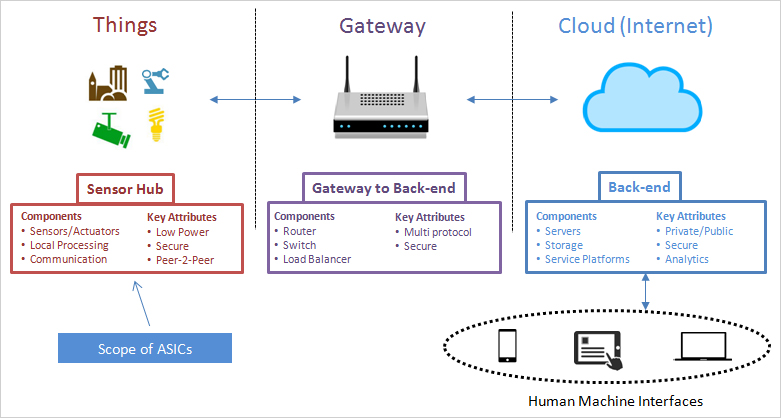
\includegraphics[scale=0.6]{image/internet-of-things1}
	\caption{Kiến trúc hệ thống IoT}
	nguồn:http://www.open-silicon.com/wp-content/uploads/2015/05/internet-of-things1.jpg
	\label{fig:iot}
\end{figure}
\subsubsection{Các giao thức trong IoT}
Điều quan trọng trong Internet of Things là các thiết bị phải được đưa lên internet, tức là phải có một định danh duy nhất. Tuy nhiên, với giao thức IPv4, số lượng định danh có thể có là hơn 4 tỷ định danh. Mặc dù có thể dùng các kỹ thuật để tăng số lượng IPv4 (ví dụ NAT, ...) tuy nhiên không thể giải quyết triệt để vấn đề này trong khi số lượng thiết bị IoT ngày càng tăng với tốc độ nhanh chóng và sẽ lên tới hàng chục tỷ thiết bị. Do đó giao thức IPv6 (có thể có hơn 2 triệu tỷ định danh) đang được tích cực triển khai để giải quyết vấn đề này. 

Một số giao thức truyền thông được sử dụng trong IoT là các giao thức truyền thông phổ biến như wifi, bluetooth, NFC, ... Tuy nhiên, cũng có các giao thức được sử dụng rộng rãi trong IoT nhưng ít được biết đến hơn như Zigbee, MQTT, AMQP, RFID,... Do tính đơn giản, dễ triển khai mà vẫn đảm bảo được các chức năng cơ bản trong môi trường IoT như gửi, nhận dữ liệu, đảm bảo chất lượng dịch vụ (QoS) nên MQTT là giao thức được sử dụng rộng rãi trong các ứng dụng IoT. Và trong đồ án này, tôi cũng sử dụng giao thức này để thực hiện gửi, nhận dữ liệu giữa các thành phần của hệ thống.\\ 
MQTT (Message Queuing Telemetry Transport) là một giao thức gửi dạng publish/subscribe sử dụng cho các thiết bị IoT với băng thông thấp, độ tin cậy cao và khả năng được sử dụng trong mạng lưới không ổn định. Trong đó, broker được coi như trung tâm, nó là điểm giao của tất cả các kết nối đến từ client. Nhiệm vụ chính của broker là nhận message (gói tin) từ publisher, xếp các message theo hàng đợi rồi chuyển chúng tới một địa chỉ cụ thể. Nhiệm vụ phụ của broker là nó có thể đảm nhận thêm một vài tính năng liên quan tới quá trình truyền thông như: bảo mật message, lưu trữ message, logs,... Client thì được chia thành 2 nhóm là publisher và subscriber. Client là các chương trình được thiết kế để có thể hoạt động một cách linh hoạt (lightweight). Client chỉ làm ít nhất một trong 2 việc là publish các message lên một topic cụ thể hoặc subscribe một topic nào đó để nhận message từ topic này. \\
Các khái niệm đáng chú ý trong giao thức MQTT:
\begin{itemize}
	\item Message: Trong giao thức MQTT, message còn được gọi là "message payload", có định dạng mặc định là plain-text (chữ viết người đọc được), tuy nhiên người sử dụng có thể cấu hình thành các định dạng khác.
	\item Topic: Topic có thể coi như một "đường truyền" logic giữa 2 điểm là publisher và subscriber. Về cơ bản, khi message được publish vào một topic thì tất cả những subscriber của topic đó sẽ nhận được message này. 
\end{itemize}

%\clearpage

\begin{figure}[h!]
	\center
	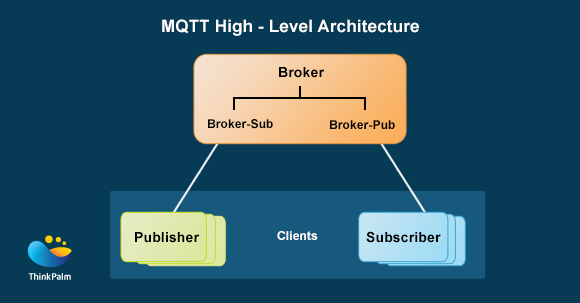
\includegraphics[scale=0.6]{image/mqtt}\\
	\caption{Giao thức truyền tin MQTT}
	Nguồn: https://techmaster.vn/posts/34394/iot-giao-thuc-mqtt-va-ung-dung-trong-iot
\end{figure} 


%Tương tự như MQTT, AMQP (Advanced Message Queuing Protocol) cũng là một giao thức dựa trên cơ chế message-queue nhưng phức tạp hơn MQTT và cung cấp các tính năng nâng cao hơn MQTT.

%Mạng không dây thế hệ thứ năm 5G hứa hẹn có tốc độ lớn hơn nhiều so với hiện tại và có khả năng kết nối đồng thời nhiều hơn các thiết bị thông minh. Mạng nhanh hơn đồng nghĩa với việc dữ liệu từ các thiết bị thông minh sẽ được thu thập, phân tích và xử lý với cấp độ cao hơn. Đây sẽ là nguồn năng lượng sáng tạo cho các công ty tạo ra các thiết bị IoT và thúc đẩy nhu cầu của khách hàng cho các sản phẩm mới. 

\subsubsection{Các nền tảng IoT}
Theo \cite{iotplatform}, nền tảng IoT là một phần mềm giúp hỗ trợ quản lý các thiết bị, giúp đơn giản hóa việc giao tiếp, luồng dữ liệu, quản lý thiết bị và các chức năng của các ứng dụng. Nó đóng vai trò là lớp trung gian giữa tầng thiết bị và tầng ứng dụng. Công việc chủ yếu của nó bao gồm thu thập dữ liệu từ thiết bị thông qua các giao thức, mô hình mạng khác nhau, điều khiển và cấu hình các thiết bị. 
\clearpage

\begin{figure}[h!]
	\center
	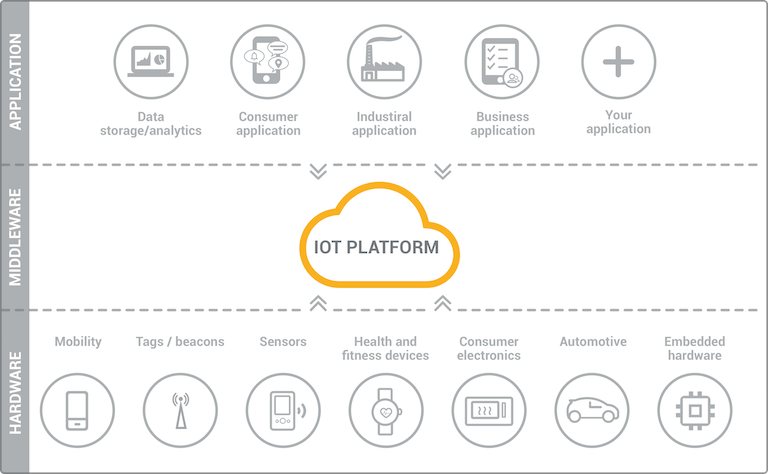
\includegraphics[scale=0.6]{image/IoTPlatform}
	\caption{Nền tảng IoT}
	Nguồn: https://www.kaaproject.org/uploads/2016/12/WhatisIoTPlatform\_05-768x474.png
	\label{fig:iot-platform}
\end{figure}


Một số nền tảng IoT đóng được dùng phổ biến như Google Cloud Platform, Saleforce IoT Cloud, IBM Wastson IoT, AWS IoT, ... Ngoài ra, các cộng đồng mã nguồn mở cũng có một số nền tảng IoT phổ biến như OpenHAB, HomeAssistant, ThingsBoard, …

%\subsection{Bảo mật và an toàn trong IoT}
%Vấn đề bảo mật trong IoT đã trở thành một chủ đề thu hút được nhiều sự chú ý sau một loạt các vụ tấn công nghiêm trọng có liên quan tới các thiết bị IoT được sử dụng để xâm nhập và tấn công các mạng máy tính lớn. Việc thực hiện các biện pháp bảo mật đóng vai trò hết sức quan trọng trong việc đảm bảo mạng các thiết bị IoT được kết nối tới nhau an toàn.

%Có một số thách thức ngăn cản sự bảo mật của các thiết bị IoT và đảm bảo bảo mật cho toàn bộ môi trường IoT. Ý tưởng về việc kết nối các thiết bị và các vật thành một mạng vẫn còn tương đối mới, do đó vấn đề bảo mật không phải luôn được xem như là ưu tiên trong suốt quá trình thiết kế sản phẩm. Thêm vào đó, vì IoT là một thị trường mới, nhiều nhà thiết kế sản phẩm và các công ty quan tâm tới việc đưa sản phẩm của họ ra thị trường hơn việc xây dựng cơ chế bảo mật ngay từ đầu. Vấn đề chính được nêu ra với việc bảo mật trong IoT là việc sử dụng các mật khẩu mặc định, có thể dẫn tới sự xâm nhập an ninh trái phép và dù mật khẩu được đổi, chúng lại thường không đủ mạnh để ngăn chặn truy nhập trái phép. Một vấn đề phổ biến khác là các thiết bị IoT thường bị giới hạn về tài nguyên và không đủ năng lực tính toán cần thiết để cài đặt hệ thống bảo mật mạnh. Do đó, rất nhiều thiết bị không hoặc không thể cung cấp các tính năng bảo mật nâng cao. Ví dụ, một cảm biến nhiệt độ, độ ẩm không thể cài đặt cơ chế mã hóa hay các cơ chế bảo mật khác. Thêm vào đó, nhiều thiết bị IoT được đặt trong một cái máy và ở đó cho tới khi không sử dụng được nữa, chúng khó lòng được cập nhật các phiên bản bảo mật mới. Từ góc nhìn nhà sản xuất, xây dựng cơ chế bảo mật từ đầu vì có thể sẽ tốn kém, làm chậm quá trình phát triển.

%Một số sự kiện về lỗ hổng, thâm nhập trái phép các thiết bị trong IoT đã được ghi nhận. Năm 2010, các nhà nghiên cứu đã phát hiện vi rút Stuxnet được sử dụng để gây thiệt hại tới các máy li tâm của Iran, các cuộc tấn công bắt đầu từ năm 2006 nhưng chủ yếu xảy ra vào năm 2009. Thường được xem là ví dụ đầu tiên của việc tấn công mạng IoT, Stuxnet nhắm vào hệ thống giám sát và thu thập dữ liệu (SCADA) với hệ thống điều khiển công nghiệp (ICS), sử dụng mã độc để đầu đọc các lệnh gửi từ bộ điều khiển logic (PLC). Các vụ tấn công vào hệ thống công nghiệp vẫn tiếp tục diễn ra, với các mã độc như CrasshOverride, Triton, VPNFilter, …
%Tháng 12 năm 2013, một nhà nghiên cứu tại công ty bảo mật Proofpoint Inc. đã mô tả mạng IoT botnet đầu tiên. Theo đó, hơn 25\% của botnet được tạo ra từ các thiết bị IoT như smart TV, hệ thống giám sát trẻ và các đồ dùng trong nhà. Năm 2015, nhà nghiên cứu bảo mật Charlie Miller và Chris Valasek đã thực hiện hack vào một xe Jeep bằng mạng không dây, điều chỉnh máy phát radio trên xe, máy lạnh và dừng cảm biến gia tốc. Họ còn nói rằng, họ có thể tắt máy, phanh xe và tắt phanh. Miller và Valasek còn có thể thâm nhập vào mạng của chiếc xe thông qua hệ thống trong chiếc xe. 
%Tháng 1 năm 2017, FDA cảnh báo hệ thống nhúng trong các thiết bị tim như máy điều hòa nhịp tim, máy khử rung tim và các thiết bị bất đồng bộ có thể bị thông nhập thông qua các lỗ hổng bảo mật.

%\subsection{Các dự đoán về IoT}
%Một số dự đoán về tương lai của IoT đã được đưa ra. Theo IoT Analytics, năm 2016 có khoảng 4.7 tỷ thiết bị, và tới năm 2021 số lượng thiết bị sẽ đạt tới 21 tỷ thiết bị. Nhờ sự phát triển của IoT, ngày càng nhiều thiết bị, nhà cửa, thành phố sẽ trở nên thông minh hơn, trong đó các thành phố sẽ có khả năng tự động một số công việc, quản lý từ xa và thu thập dữ liệu thông qua các ki-ốt, camera giám sát, các trạm cho thuê xe, ... Khi dữ liệu trở nên nhiều hơn, trí thông minh nhân tạo AI sẽ đóng vai trò quan trọng hơn. Học máy, một lĩnh vực trong AI sẽ giúp máy tính có thể "học" để đưa ra các gợi ý mang tính cá nhân hóa cao hơn. Trong lĩnh vực bảo mật, tội phạm mạng vẫn sẽ tiếp tục sử dụng các thiết bị IoT để thực hiện các cuộc tấn công DDos. Bên cạnh đó, mối quan tâm về bảo mật và quyền riêng tư sẽ dành nhiều hơn cho tính pháp lý và các quy định về dữ liệu, đảm bảo quyền bảo mật thông tin cá nhân của người dân tốt hơn.


\section{Giới thiệu về truy vấn ngữ nghĩa}
\subsection{Truy vấn ngữ nghĩa}
Truy vấn cho phép truy vấn và phân tích ngữ cảnh tự nhiên của câu truy vấn. Truy vấn ngữ nghĩa cho phép lấy ra các thông tin rõ ràng cũng như các thông tin ẩn về dữ liệu. Để xây dựng cơ chế truy vấn ngữ nghĩa, ta cần xây dựng mô hình mối quan hệ của các dữ liệu, một trong những cách để thực hiện là xây dựng ontology.

\subsection{Ontology}
\subsubsection{Khái niệm ontology}
Lịch sử của trí tuệ nhân tạo cho thấy rằng tri thức đóng vai trò hết sức quan trọng trong các hệ thống thông minh. Trong rất nhiều trường hợp, tri thức tốt có thể quan trọng hơn các giải thuật trong việc giải quyết một bài toán. Để có được một hệ thống thực sự thông minh, trí thức cần được thu thập, xử lý, tái sử dụng và được trao đổi. Ontology hỗ trợ tất cả các công việc này. Khái niệm ontology có thể được định nghĩa như sự cụ thể hóa một cách rõ ràng các khái niệm trong một miền lĩnh vực. Ontology thể hiện cấu trúc của miền lĩnh vực, bao gồm cả các mối quan hệ ràng buộc của các thành phần trong lĩnh vực đó. Các khái niệm trong một lĩnh vực thường không thay đổi hoặc rất ít thay đổi, và ontology là một bản mô tả các khái niệm trong lĩnh vực đó dựa trên ngôn ngữ mô hình hóa và các từ vựng cụ thể. Việc mô tả một cách hình thức ontology là yêu cầu bắt buộc để có thể xử lý và thực hiện các thao tác một các tự động trên ontology. Để xây dựng được ontology, ta cần xác định một cách hình thức các thành phần trong ontology như các thực thể của một khái niệm, các lớp (khái niệm), các thuộc tính của các khái niệm và mối quan hệ cũng như các ràng buộc, các luật, các tiên đề giữa các khái niệm. 

Các thực thể là một thành phần cơ bản của ontology. Các thực thể trong một ontology có thể là các đối tượng cụ thể ví dụ như một người cụ thể, một con vật cụ thể, một hành tinh cụ thể, ... 

Lớp hay khái niệm có thể được định nghĩa là một tập trừu tượng của các đối tượng. Các khái niệm có thể bao gồm các thực thể của các đối tượng hoặc cũng có bao gồm loại các khái niệm khác. Ví dụ, "động vật" là một khái niệm chỉ chung các cá thể động vật như chim, cá, hổ, báo, sư tử, con người, ... "Con người" lại có thể là một khái niệm chỉ tất cả những người sống trên Trái Đất. 

Các đối tượng trong một ontology có thể được mô tả bởi liên kết chúng tới các thành phần, các khía cạnh, ... của nó. Những thành phần, khía cạnh này được gọi là các thuộc tính tính. Mỗi thuộc tính cũng có thể là một lớp hay một thực thể. Ví dụ, "con người" có thể có thuộc tính "giới tính", "tên", "tuổi", ...
 
Mối quan hệ giữa các khái niệm trong một ontology xác định xem khái niệm này có liên quan tới khái niệm khác như thế nào. Ví dụ, khái niệm "con người" có mối quan hệ "là một loài" với khái niệm "động vật". Biểu diễn trở thành: "con người" là một loài "động vật". \\
Sức mạnh của ontology đến từ khả năng miêu tả các mối quan hệ giữa các khái niệm. Tập các mối quan hệ sẽ mô tả tính ngữ nghĩa của lĩnh vực. Một loại quan hệ rất quan trọng trong ontology là mối quan hệ: một khái niệm là khái niệm cha của một khái niệm khác. Ví dụ, "ô tô" là khái niệm cha của "ô tô bốn bánh". Ngược lại với mối quan hệ trên là mối quan hệ: một khái niệm là khái niệm con của một khái niệm khác. Ví dụ, "ô tô bốn bánh" là khái niệm con của "ô tô". Một mối quan hệ thường dùng khác là mối quan hệ: một khái niệm là một phần của một khái niệm khác. Ví dụ, "bánh xe", "cửa sổ" là một phần của "ô tô". 

Tập luật  là các mệnh đề dưới dạng điều kiện - kết quả (nếu-thì), dùng để mô tả phép suy dẫn logic từ một tập các mối quan hệ. Ví dụ, "nếu" "cá voi" là một loài "động vật"  và "động vật" là một loài "sinh vật" "thì" "cá voi" là một loài sinh vật.

Các tiên đề là các khẳng định mang tính logic. Ví dụ "memo" là một "con cá" và "mọi con cá" đều biết bơi nên "memo" biết bơi. 

\clearpage
\begin{figure}
	\center
	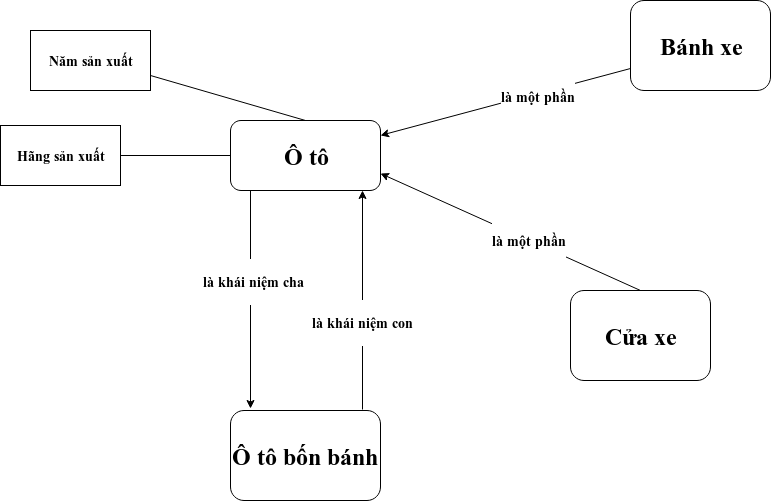
\includegraphics[scale=0.6]{image/otology_example}
	\label{fig:ontology}
	\caption{Một ví dụ về ontology}
\end{figure}


Ontology không chỉ là bản mô tả có thể chia sẻ và tái sử dụng của một lĩnh vực mà còn có thể thêm các tri thức mới về lĩnh vực đó. 
Có một số cách khác có thể được sử dụng để mô tả một cách hình thức tri thức về một miền lĩnh vực như cơ sở dữ liệu quan hệ, sử dụng tập từ vựng của lĩnh vực, ... tuy nhiên, ontology nhấn mạnh mối quan hệ giữa các khái niệm và cho phép người sử dụng liên kết các khái niệm này với các khái niệm khác theo nhiều cách khác nhau. 
\subsubsection{Cách xây dựng một ontology}
Có nhiều phương pháp để xây dựng một ontology, tuy nhiên, nhìn chung, các phương pháp đều thực hiện hai bước cơ bản: xây dựng cấu trúc lớp phân cấp và định nghĩa các thuộc tính cho các lớp. Trong thực tế, để xây dựng một ontology mô tả một lĩnh vực là một công việc khó khăn, phụ thuộc rất nhiều vào công cụ sử dụng, tính chất, quy mô, sự thường xuyên biến đổi của lĩnh vực đó, cũng như các mối quan hệ phức tạp trong đó. Những khó khăn này đòi hỏi quá trình xây dựng ontology phải là một quá trình lặp đi lặp lại, mỗi lần lặp cải thiện, tinh chế và phát triển dần sản phẩm chứ không phải là một quy trình với các công đoạn tách rời nhau. Công việc xây dựng ontology cũng cần phải tính đến khả năng mở rộng lĩnh vực quan tâm trong tương lai, khả năng kế thừa các ontology đã có, cũng như có tính linh động để ontology có khả năng mô tả tốt nhất các mối quan hệ phức tạp trong thế giới thực. 
Một số nguyên tắc cơ bản trong xây dựng ontology:
\begin{itemize}
	\item Không có một cách duy nhất nào để mô hình hóa một lĩnh vực. Luôn có rất nhiều cách có thể thay thế cho nhau. Việc xác định cách tốt nhất thường phụ thuộc vào ứng dụng của mô hình và các mở rộng trong tương lai mà ta đoán trước sẽ có thể xảy ra.
	\item Quá trình phát triển ontology là một quá trình lặp đi lặp lại
	\item Các khái niệm trong ontology nên sát với các đối tượng (vật lý hoặc logic) trong lĩnh vực mà nó mô tả. Các khái niệm thường là những danh từ, các mối quan hệ thường là những động từ được dùng trong lĩnh vực.
\end{itemize}

Do đó, việc quyết định xem ontology dùng để làm gì và mức độ chi tiết hay tổng quát của ontology sẽ ảnh hưởng tới các quyết định trong khi xây dựng ontology. Trong rất nhiều các lựa chọn, chúng ta phải xác định lựa chọn nào sẽ phù hợp nhất với mục đích của ứng dụng, lựa chọn nào sẽ giúp ontology có khả năng mở rộng và có tính ổn định cao. Chúng ta cũng cần nhớ rằng một ontology là một bản mô tả một phần của thế giới và các khái niệm trong ontology phải phản ánh được phần thế giới đó. Sau khi ta đã tạo ra được một phiên bản đầu tiên của một ontology, ta có thể đánh giá, sửa đổi nó dựa trên ứng dụng sử dụng nó,  dựa trên ý kiến của các chuyên gia trong lĩnh vực,... Quá trình sửa đổi này sẽ tiếp tục cho tới hết vòng đời sử dụng của ontology.
Theo \cite{howtocreateontology1}, \cite{howtocreateontology2}, việc xây dựng ontology cần thực hiện các bước sau:

\underline{Bước 1:} Xác định lĩnh vực và phạm vi của ontology

Thông thường, các yêu cầu đối với một hệ thống Ontology là mô tả lĩnh vực quan tâm nhằm phục vụ cơ sở tri thức trong việc giải quyết những mục đích chuyên biệt. Công việc đặc tả để xác định, phân tích, nhận diện chính xác yêu cầu được thực hiện bằng cách trả lời những câu hỏi sau:
\begin{itemize}
	\item Ontology cần mô tả lĩnh vực nào?
	\item Mục đích sử dụng ontology là gì?
	\item Cơ sở tri thức trong Ontology sẽ giải quyết những câu hỏi gì?
	\item Ai là người sẽ xây dựng, quản trị Ontology?
\end{itemize}
Nhìn chung, câu trả lời cho các câu hỏi dạng này có thể sẽ thường xuyên thay đổi trong suốt quá trình xây dựng một Ontology. Nhất là khi có sự thay đổi về mục đích hoặc cần bổ sung tính năng trong việc sử dụng cơ sở tri thức. Tuy nhiên, việc trả lời chính xác các câu hỏi trên tại mỗi bước lặp sẽ giúp giới hạn phạm vi của mô hình cần mô tả và dự trù các kỹ thuật sẽ sử dụng trong quá trình phát triển. Lấy ví dụ, nếu dự trù khả năng xảy ra sự khác biệt về ngôn ngữ giữa người phát triển và người sử dụng thì Ontology phải được bổ sung cơ chế ánh xạ (mapping) qua lại các thuật ngữ giữa các ngôn ngữ khác nhau. Hoặc giả sử Ontology cần xây dựng có chức năng xử lý ngôn ngữ tự nhiên, ứng dụng dịch tài liệu tự động thì cũng cần thiết phải có kỹ thuật xác định từ đồng nghĩa. Sau khi đã phác thảo phạm vi ontology dựa trên việc trả lời những câu hỏi trên, người thiết kế sẽ trả lời các câu hỏi mang tính đánh giá, qua đó tiếp tục tinh chỉnh lại phạm vi của hệ thống cần xây dựng. Các câu hỏi dạng này thường dựa trên cơ sở tri thức của Ontology và được gọi là câu hỏi kiểm chứng khả năng (competency question):
\begin{itemize}
	\item Ontology đã có đủ thông tin để trả lời cho các câu hỏi được quan tâm trên cơ sở tri thức hay không?
	\item Câu trả lời của cơ sở tri thức đã đáp ứng được mức độ, yêu cầu nào của người sử dụng?
	\item Các ràng buộc và quan hệ phức tạp trong miền quan tâm đã được biểu diễn hợp lý chưa? 
\end{itemize}
\underline{Bước 2:} Xem xét việc kế thừa các ontology có sẵn: \\
Đây là một công đoạn thường hay sử dụng để giảm thiểu công sức xây dựng một Ontology. Bằng cách kế thừa các ontology tương tự có sẵn, người xây dựng có thể thêm hoặc bớt các lớp, quan hệ giữa các lớp, thực thể để tinh chỉnh tùy theo mục đích của mình. Việc sử dụng lại các Ontology có sẵn cũng rất quan trọng khi cần sự tương tác giữa các ứng dụng khác nhau, các ứng dụng sẽ cần phải hiểu các lớp, thực thể, quan hệ của nhau để thuận tiện trong việc trao đổi hoặc thống nhất thông tin.\\

Trong các ontology về IoT, SSN ontology \cite{ssnontology} là ontology được nhắc đến rất phổ biến. Ontology này mô tả các cảm biến, các quan sát và các khái niệm liên quan. Nó không mô tả các thành phần như thời gian, địa điểm, ... Những thành phần này, có thể được thêm vào từ các ontology khác thông qua ngôn ngữ OWL (Web Ontology Language).
SSN ontology được phát triển bởi W3C Semantic Sensor Network Incubator Group (SSN-XG). Việc thiếu các khái niệm để mô tả cụ thể các loại cảm biến, đơn vị của các giá trị thu được, thời gian, địa điểm, ... khiến cho SSN ontology khó tích hợp được vào các lĩnh vực cụ thể mà đôi khi không theo chuẩn chung.
%\clearpage

\begin{figure}[h!]
	\center
	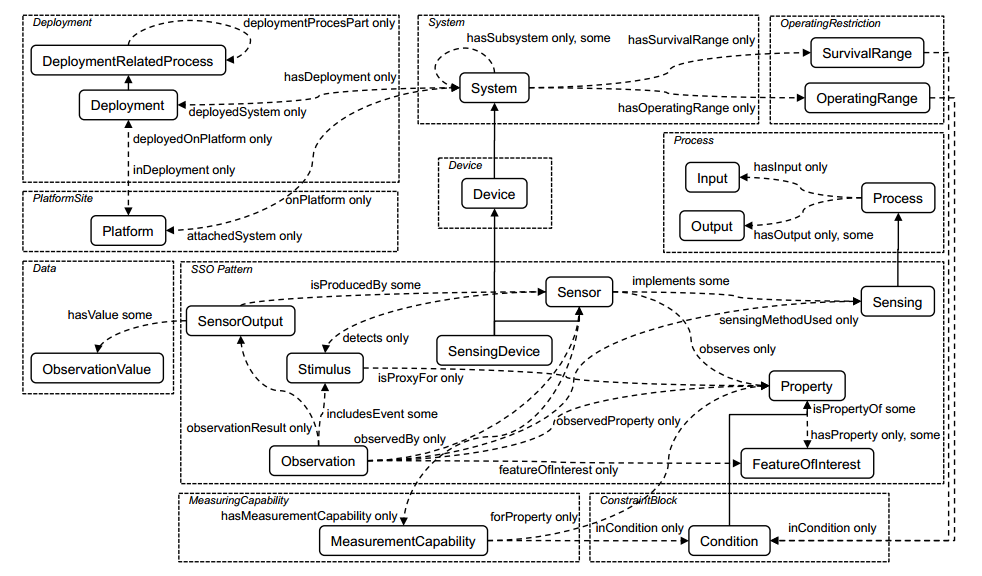
\includegraphics[scale=0.5]{image/ssn_ontology} \\
	\caption{SSN ontology}
	\small nguồn: https://corescholar.libraries.wright.edu/knoesis/610/?utm\_source=corescholar.libraries.wright.edu \%2Fknoesis\%2F610\&utm\_medium=PDF\&utm\_campaign=PDFCoverPages
\end{figure}

Một ontology khác là ontology IoT-A \cite{iotaontology}, cung cấp các khái niệm chính như Service, và các khái niệm chủ yếu theo liên quan tới các Service. Nó chỉ tái sử dụng khái niệm ssn:condition. Hơn nữa, nó rất phức tạp, không sử dụng các ontology chuẩn, và gặp nhiều vấn đề về tính dư thừa. 
%\clearpage

\begin{figure}[h!]
	\center
	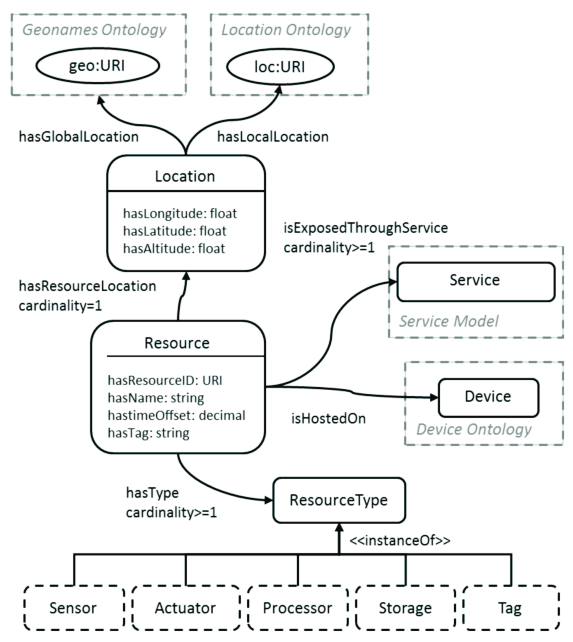
\includegraphics[scale=0.6]{image/iot-a}
	\caption{IoT-A ontology}
	nguồn: https://www.researchgate.net/profile/Suparna\_De/publication/330729011/figure/fig1/ AS:720756187090946@1548853074205/Internet-of-Things-Architecture-IoT-A-Resource-Model.png
\end{figure}

IoT-Lite ontology \cite{iotliteontology} là một ontology rút gọn của SSN ontology để biểu diễn các tài nguyên, thực thể và các dịch vụ trong IoT. Sự rút này cho phép IoT-Lite không quá lớn và không cần thời gian dài để xử lý khi thực hiện một truy vấn trên ontology này. Tuy nhiên, nó cũng cho phép khả năng mở rộng để biểu diễn các khái niệm trong IoT một cách chi tiết hơn, trong các lĩnh vực khác. Nó cũng có thể được kết hợp với các ontology biểu diễn dữ liệu IoT dạng stream như SAO ontology. 
\clearpage

\begin{figure}[h!]
	\center
	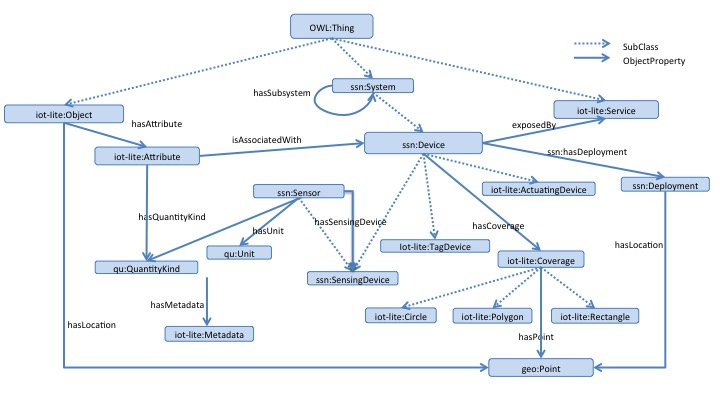
\includegraphics[scale=0.6]{image/iot-lite} \\
	\caption{IoT-Lite ontology}
	nguồn: https://www.w3.org/Submission/2015/SUBM-iot-lite-20151126/figures/Ontology.jpg
\end{figure}

\underline{Bước 3:} Liệt kê các thuật ngữ quan trọng trong Ontology:\\
Đây là bước rất hữu ích, làm tiền đề cho hai bước tiếp theo là xây dựng cấu trúc lớp phân cấp và định nghĩa các thuộc tính cho lớp. Công đoạn này bắt đầu bằng việc liệt kê tất cả các thuật ngữ xuất hiện trong miền quan tâm (có thể đồng nghĩa hoặc chồng nhau)như tên khái niệm, quan hệ, thuộc tính. Thông thường, các thuật ngữ là danh từ sẽ trở thành các lớp, tính từ sẽ trở thành thuộc tính, còn động từ sẽ là quan hệ giữa các lớp. 

\underline{Bước 4:} Xây dựng các lớp/khái niệm và cấu trúc lớp/khái niệm phân cấp:\\
Đây là một trong hai bước quan trọng nhất của công việc xây dựng một Ontology. Nhiệm vụ của bước này là định nghĩa các lớp từ một số thuật ngữ đã liệt kê trong bước trên, sau đó xây dựng cấu trúc lớp phân cấp theo quan hệ lớp cha-lớp con. Lớp ở vị trí càng cao sẽ có mức độ tổng quát càng cao. Vị trí đầu tiên thuộc về lớp gốc, tiếp theo là các lớp trung gian, và cuối cùng là lớp lá. Lớp lá là lớp không thể triển khai được nữa và chỉ được biểu hiện bằng các thực thể. Quan hệ giữa thực thể của lớp con với lớp cha là quan hệ "là một", nghĩa là một thực thể của lớp con cũng “là-một” thực thể của lớp cha. Có nhiều hướng tiếp cận khác nhau cho vấn đề xây dựng cấu trúc lớp phân cấp. Có thể kể ra ba hướng như sau: 
\begin{itemize}
	\item Hướng xây dựng từ trên xuống (top-down): bắt đầu bằng các lớp có mức độ tổng quát cao nhất, sau đó triển khai dần đến lớp lá.
	\item Hướng xây dựng từ dưới lên (bottom-up): ngược với hướng xây dựng cấu trúc lớp phân cấp từ trên xuống, hướng này bắt đầu bằng việc xác định các lớp được cho là cụ thể nhất, sau đó tổng quát hóa đến khi được lớp gốc.
	\item Cách kết hợp (combination): cách này kết hợp cả hai hướng xây dựng trên. Đầu tiên chọn các lớp nổi bật nhất trong lĩnh vực quan tâm, sau đó tổng quát hóa và cụ thể hóa cho đến khi được cấu trúc mong muốn.
\end{itemize}

Không có phương pháp nào trong ba phương pháp này là tốt nhất trong mọi trường hợp. Việc lựa chọn phương pháp nào phụ thuộc vào góc nhìn cá nhân của người xây dựng vào lĩnh vực. Nếu người xây dựng có một cái nhìn hệ thống từ trên xuống thì phương pháp xây dựng từ trên xuống sẽ phù hợp. Ngược lại, một người có cái nhìn từ dưới lên sẽ phù hợp với cách xây dựng từ dưới lên. Phương pháp kết hợp thường là cách dễ nhất cho những người xây dựng. 

\underline{Bước 5:} Định nghĩa các thuộc tính và quan hệ cho lớp: \\
Bản thân các lớp nhận được ở bước trên chỉ mới là những thuật ngữ phân biệt với nhau bằng tên gọi. Về cơ bản, chúng chưa đủ để phục vụ cho việc biểu diễn tri thức. Muốn như vậy, các thuộc tính của lớp cần được định nghĩa. Thuộc tính của lớp là các thông tin bên trong của lớp, mô tả một khía cạnh nào đó của lớp và được dùng để phân biệt với các lớp khác. Thuộc tính được chia làm nhiều loại khác nhau:
Về mặt ý nghĩa, các thuộc tính có thể được chia làm hai loại: thuộc tính bên trong
(intrinsic property) và thuộc tính bên ngoài (extrinsic property). Thuộc tính bên trong mô tả các tính chất nội tại bên trong sự vật, ví dụ: chất, lượng, cấu tạo. Trong khi đó, thuộc tính bên ngoài mô tả phần biểu hiện của sự vật, ví dụ: màu sắc, hình dạng. Về mặt giá trị, các thuộc tính cũng được chia làm hai loại: thuộc tính đơn (simple property) và thuộc tính phức (complex property). Thuộc tính đơn là các giá trị đơn, ví dụ: chuỗi, số,.. còn thuộc tính phức có thể chứa hoặc tham khảo đến một đối tượng khác. Một chú ý quan trọng nữa trong bước này là việc một lớp sẽ kế thừa toàn bộ các thuộc tính của tất cả các cha nó. Do đó cần phải xem xét một thuộc tính đã được định nghĩa ở các lớp thuộc mức cao hơn hay chưa. Thuộc tính chỉ nên được định nghĩa khi nó là tính chất riêng của lớp đang xét mà không được biểu hiện ở các lớp cao hơn. 

\underline{Bước 6:} Định nghĩa các ràng buộc của các thuộc tính \\
Các thuộc tính có thể có các ràng buộc như kiểu giá trị, miền giá trị, số lượng giá trị và các ràng buộc khác. Ví dụ, một tên phải là một chuỗi các chữ cái, do đó, thuộc tính "tên" phải có ràng buộc là một chuỗi (string). 
Một số ràng buộc của các thuộc tính thường gặp:
\begin{itemize}
	\item Số lượng giá trị: Xác định một thuộc tính có thể có bao nhiêu giá trị. Một vài thuộc tính chỉ có thể có một giá trị, ví dụ thuộc tính "mã số sinh viên" của khái niệm "sinh viên" chỉ có thể nhận một giá trị. Một số thuộc tính lại có thể nhận nhiều giá trị, ví dụ thuộc tính "số điện thoại" của khái niệm "sinh viên" có thể nhận nhiều giá trị.
	\item Kiểu giá trị: Xác định loại giá trị nào mà thuộc tính có thể nhận. Một số kiểu giá trị thường gặp như:
	\begin{itemize}
		\item Chuỗi (string): là kiểu giá trị đơn giản nhất, được dùng cho các thuộc tính như "tên", "quê quán", …
		\item Số (Number): đôi khi có thể được phân nhỏ thành số nguyên và số thực, xác định thuộc tính dạng số, ví dụ như "tuổi", "số lượng", "giá", ...
		\item Đúng-sai (boolean): đơn giản chỉ nhận hai giá trị đúng hoặc sai. Kiểu giá trị này thường được dùng cho các thuộc tính như "giới tính", …
		\item Liệt kê (enumerated): liệt kê các giá trị mà thuộc tính có thể nhận. Ví dụ, "kích cỡ" có thể nhận các giá trị to, trung bình, nhỏ.
	\end{itemize}
	\item Miền giá trị: Xác định miền giá trị mà thuộc tính có thể có. Ví dụ "nhiệt độ phòng" có thể có miền giá trị từ 0 đến 100 oC.  
\end{itemize}

\underline{Bước 7:} Tạo ra các thực thể
 
Đây là bước cuối cùng khép lại một vòng lặp xây dựng Ontology. Công việc chính lúc này là tạo thực thể cho mỗi lớp và gán giá trị cho các thuộc tính. Nhìn chung, các thực thể sẽ tạo nên nội dung của một cơ sở tri thức. 


\subsubsection{Ngôn ngữ ontology}
Ngôn ngữ Ontology là ngôn ngữ hình thức được sử dụng để xây dựng ontology. Nó cho phép việc mã hóa tri thức trong một lĩnh vực cụ thể và thường bao gồm các quy tắc suy luận cung cấp cho việc xử lý các yêu cầu dựa trên tri thức đó. Ngôn ngữ ontology thường là ngôn ngữ khai báo, và hầu hết là những sự tổng hợp của ngôn ngữ cấu trúc. Có rất nhiều ngôn ngữ Ontology đã được thiết kế và đưa ra tuân theo sự tiêu chuẩn hóa, và một trong số những ngôn ngữ được sử dụng thông dụng hiện nay là RDF. Thông tin biểu diễn theo mô hình RDF là một phát biểu (statement) ở dạng cấu trúc bộ ba gồm ba thành phần cơ bản là: đối tượng, thuộc tính hay quan hệ, giá trị. Trong đó:
\begin{itemize}
	\item Đối tượng: chỉ đối tượng đang được mô tả đóng vai trò là chủ thể.
	\item Thuộc tính hay đối tượng là thuộc tính hay quan hệ của đối tượng.
	\item Giá trị: giá trị thuộc tính hay đối tượng của chủ thể đã nêu. Giá trị có thể là một giá trị nguyên thủy như số nguyên, chuỗi, …
\end{itemize}
Ví dụ: Sinh viên có tuổi là 20 được hiểu là một phát biểu đối tượng sinh viên, có thuộc tính là có tuổi là và giá trị là 20.
Có thể liệt kê một số ưu điểm của việc lưu trữ dữ liệu RDF so với dữ liệu truyền thống là: 
Tổ chức dữ liệu đơn giản, đồng nhất nên thông tin dễ dàng thêm bớt chỉnh sửa.
Cấu trúc bộ ba giúp cho thông tin dễ truy xuất bởi các hệ thống suy luận, tìm kiếm ngữ nghĩa. Cũng nhờ vậy mà những bộ xử lý RDF có thể suy luận ra những thông tin mới không có trong hệ dữ liệu. \\
Chia sẻ dữ liệu trên mạng dễ dàng nhờ sự đồng nhất. Ngoài RDF, còn có một số ngôn ngữ ontology được dùng khá phổ biến khác như RDFS, OWL,... để mô tả các tài nguyên trên môi trường web.

\subsection{Định hướng giải pháp}
Sau khi đã tìm hiểu cơ sở lý thuyết và các công nghệ liên quan, tôi quyết định sử dụng các công nghệ sau để xây dựng hệ thống IoT và cơ chế truy vấn ngữ nghĩa: 

\begin{itemize}
	\item Sử dụng các cảm biến phổ biến, dễ mua trên thị trường là cảm biến nhiệt độ-độ ẩm, cảm biến chuẩn động và các đèn LED để xây dựng hệ thống phần cứng
	\item Sử dụng giao thức MQTT là giao thức phổ biến trong môi trường IoT để gửi, nhận các thông điệp giữa thành phần trong hệ thống
	\item Các nền tảng IoT mã nguồn mở được sử dụng do dễ tiếp cận, cài đặt. Trong đồ án này, tôi sử dụng các nền tảng IoT mã nguồn mở OpenHAB, HomeAssistant và ThingsBoard. Trong đó, hệ thống ban đầu sẽ gồm hai nền tảng IoT là OpenHAB và HomeAssistant; nền tảng IoT ThingsBoard sẽ được tích hợp vào hệ thống sau này để chứng minh khả năng mở rộng của hệ thống
	\item Xây dựng ontology dựa trên bảy bước như đã nêu trong phần giới thiệu về ontology. Sử dụng định dạng json để biểu diễn các khái niệm, thuộc tính, cũng như mối quan hệ giữa các khái niệm.
\end{itemize}
\newcommand{\blank}[1]{\hspace*{#1}\linebreak[0]}
\chapter{Xây dựng hệ thống IoT và thiết kế cơ chế truy vấn ngữ nghĩa}

\section{Xây dựng hệ thống IoT}
\subsection{Phần cứng}

Các thiết bị IoT được cài đặt trên 3 khu vực trong phòng 609 thư viện Tạ Quang Bửu. Trong mỗi phòng, có một máy tính nhỏ Raspberry Pi 3, cài đặt nền tảng IoT để quản lý các thiết bị trong phòng. Trong mỗi phòng, gồm :
\begin{itemize}
	\item Một cảm biến chuyển động
	\item Một cảm biến ánh sáng
	\item Một cảm biến nhiệt độ, độ ẩm
	\item Ba đèn LED tượng trưng cho ba thiết bị IoT có khả năng thiết lập các trạng thái khác nhau (bật/tắt).
\end{itemize}
Các cảm biến và đèn LED trong mỗi phòng được cài đặt vào hai hộp đại diện cho hai thiết bị thông minh. Thiết bị thứ nhất chứa cảm biến chuyển động và ba đèn LED; thiết bị thứ hai chứa cảm biến ánh sáng, cảm biến nhiệt độ-độ ẩm. 
\clearpage

\begin{figure}
	\center
	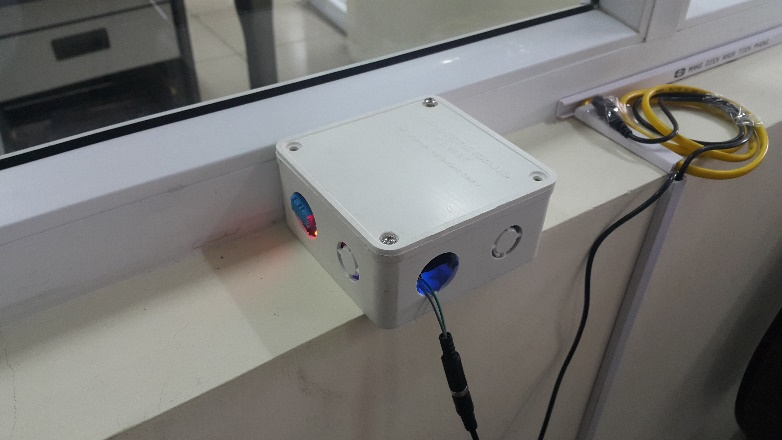
\includegraphics[scale=1]{image/hop_1}
	\label{fig:2hop}
	%\caption{Hai hộp đại diện cho hai "vật"}
\end{figure}

\begin{figure}
	\center
	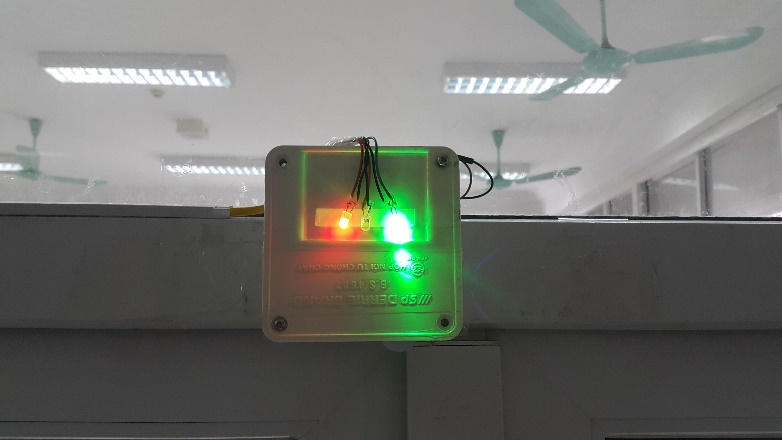
\includegraphics[scale=1]{image/hop_2}
	\label{fig:2hop}
	\caption{Hai hộp đại diện cho hai thiết bị thông minh}
\end{figure}

Để lấy được dữ liệu từ các thiết bị trên, ta sử dụng board vi mạch xử lý Arduino Uno. Tuy nhiên, vi mạch này không có chức năng gửi dữ liệu thông qua mạng wifi, do đó, cần phải lắp thêm module ESP8266 để gửi dữ liệu từ Arduino, qua ESP8266 rồi gửi lên platform.

\subsection{Các giao thức sử dụng}
Giao thức được dùng để truyền tải dữ liệu từ ESP8266 lên nền tảng IoT là MQTT thông qua mạng wifi. Sau khi đã xác định được các thành phần phần cứng và giao thức sử dụng để truyền tin giữa các thiết bị tới nền tảng IoT, tôi xây dựng mô hình triển khai như sau: \\

\clearpage
\begin{figure}[h!]
	\center
	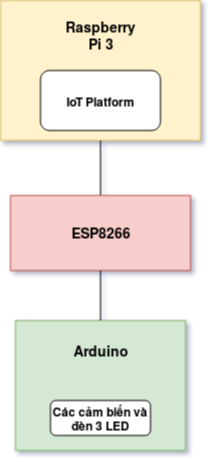
\includegraphics[scale=0.6]{image/mo_hinh_trien_khai_phan_cung}
	\caption{Mô hình triển khai hệ thống}
	
	\label{fig:mo_hinh_trien_khai_phan_cung}
\end{figure}

Hệ thống triển khai thực tế :\\

\begin{figure}[h!]
	\center
	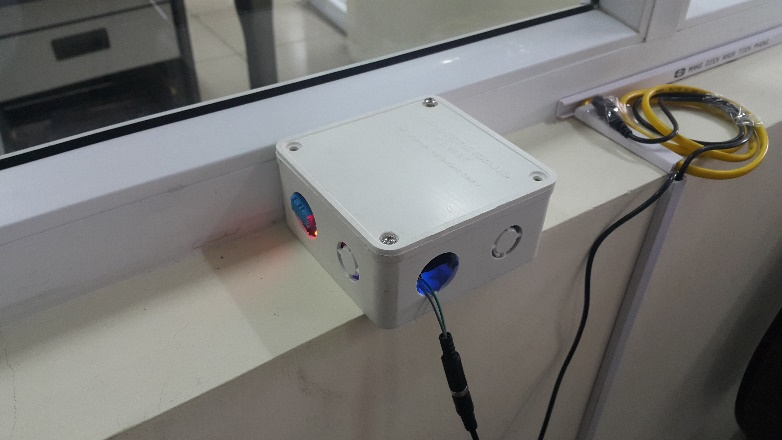
\includegraphics[scale=1]{image/hop_1}
	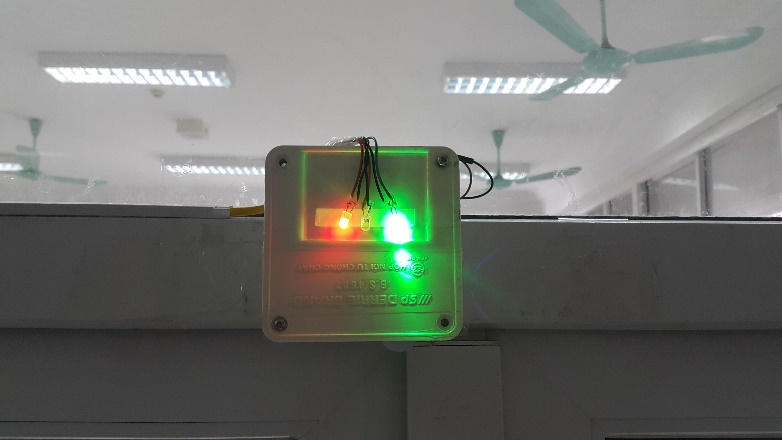
\includegraphics[scale=1]{image/hop_2}
\end{figure}

\begin{figure}[h!]
	\center
	%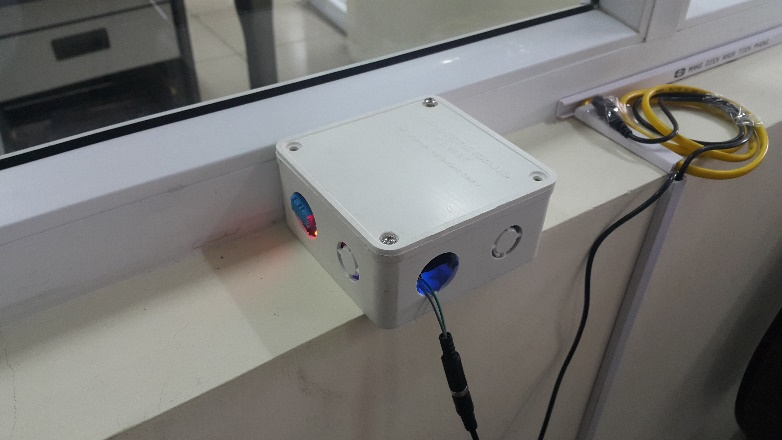
\includegraphics[scale=1]{image/hop_1}
	%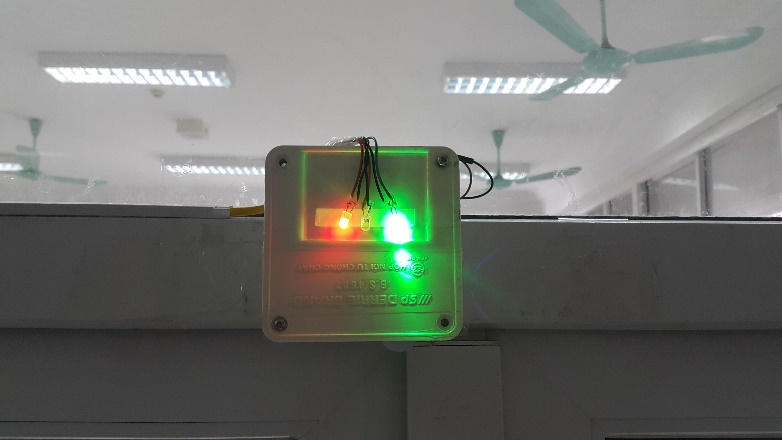
\includegraphics[scale=1]{image/hop_2}
	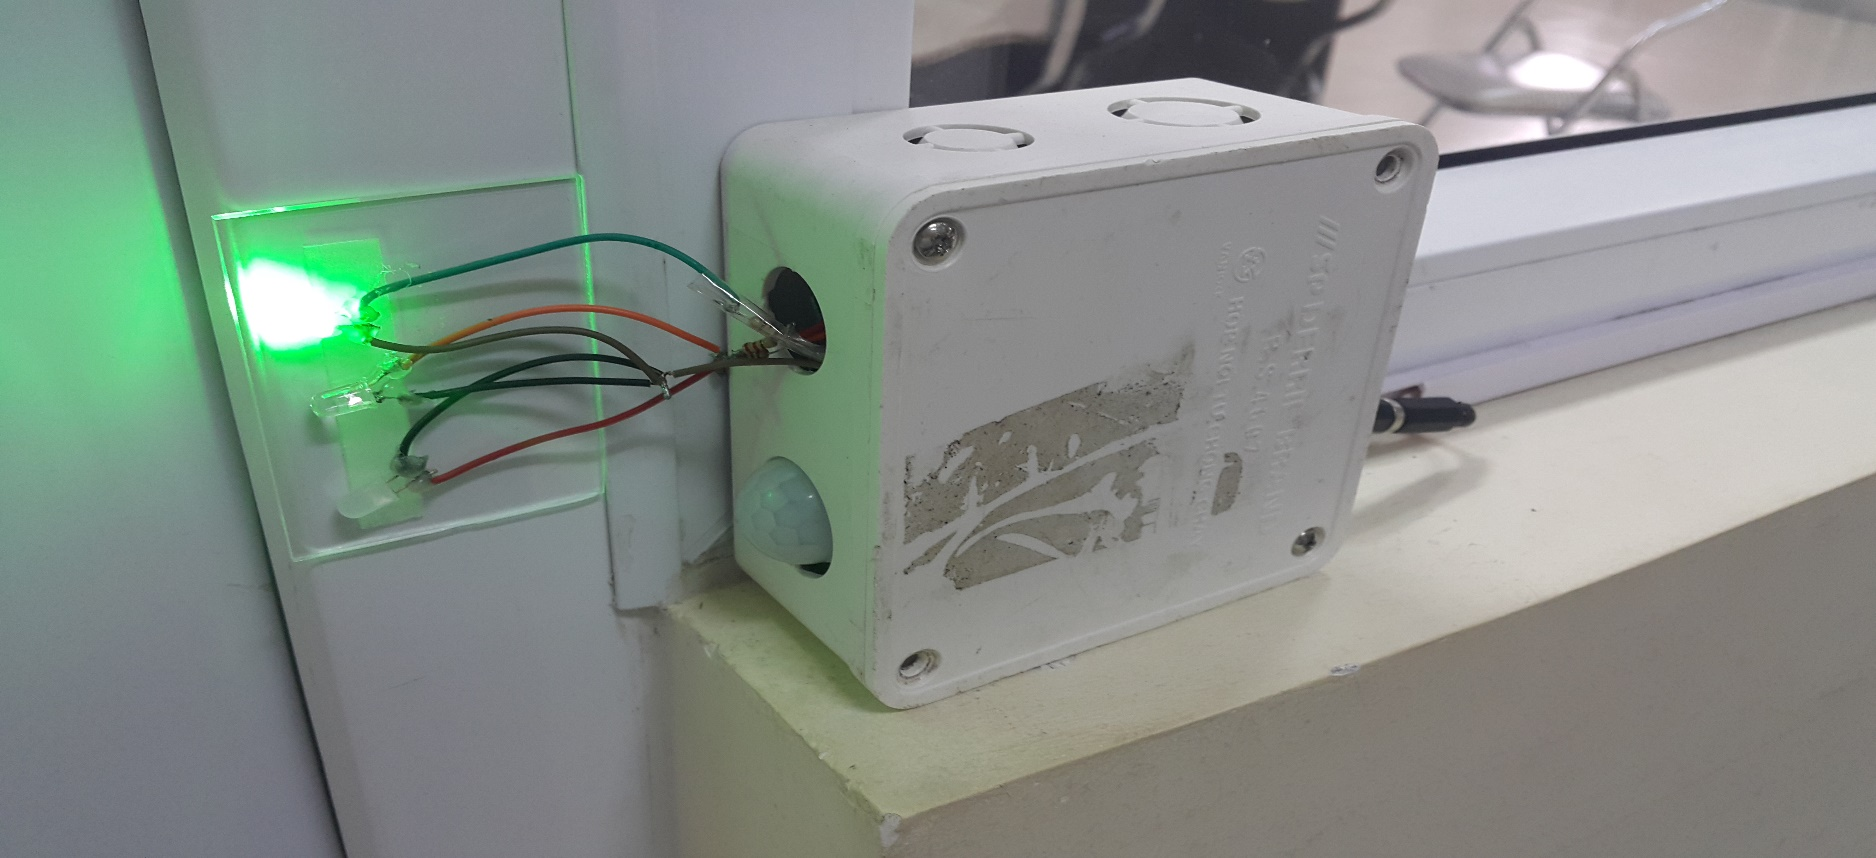
\includegraphics[scale=0.4]{image/hop_3}	
	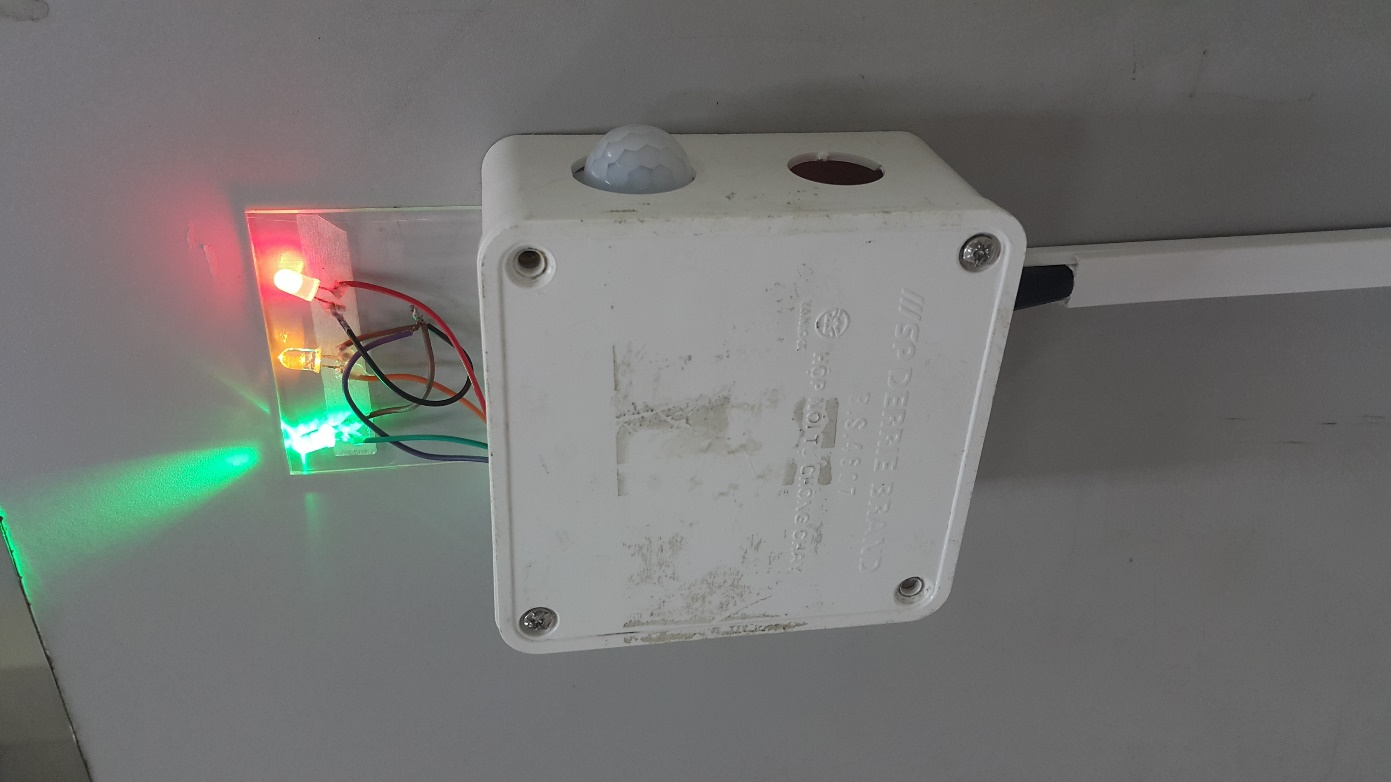
\includegraphics[scale=0.5]{image/hop_4}
	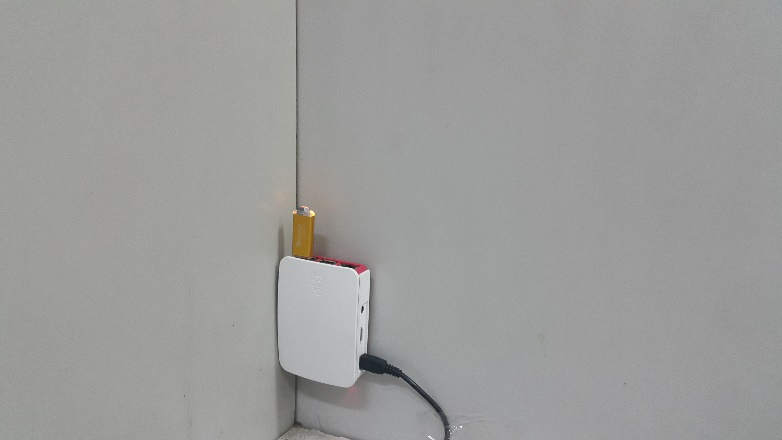
\includegraphics[scale=1]{image/hop_5}
	\caption{Triển khai phần cứng trên phòng 609 Thư viện TQB}
	\label{fig:trien_khai_phan_cung}
\end{figure}
%\clearpage 


\subsection{Các nền tảng IoT sử dụng}
Hiện nay, trong thực tế có rất nhiều các nền tảng IoT được sử dụng, cả các platform nguồn đóng và nguồn mở. Các nền tảng IoT mã nguồn đóng thường được các công ty hoạt động vì lợi nhuận xây dựng, ví dụ như IBM, Amazon, ... còn các nền tảng IoT mã nguồn mở thường được cộng đồng mã nguồn mở hoặc các công ty hoạt động phi lợi nhuận xây dựng. Do đề tài chỉ mang mục đích nghiên cứu, nên tôi sử ba nền tảng IoT mã nguồn mở để mô tả tính không đồng nhất về cấu trúc dữ liệu của các platform và cách ánh xạ các cấu trúc không đồng nhất này về dạng chuẩn chung của ontology. Ba platform được sử dụng là OpenHAB, HomeAssistant và ThingsBoard.

OpenHAB là một nền tảng IoT được dùng chủ yếu để quản lý các thiết bị trong ngôi nhà thông minh. Các ưu điểm của OpenHAB là:
\begin{itemize}
	\item Có khả năng tích hợp các thiết bị, hệ thống khác.
	\item Cung cấp giao diện thống nhất cho người dùng và người dùng có thể tạo ra các luật dựa trên thông tin của các thiết bị trong hệ thống.
	\item Cung cấp một công cụ linh động để tạo ra một ngôi nhà tự động. OpenHAB hỗ trợ tự thêm rất nhiều loại thiết bị, giao thức phổ biến trong IoT. 
\end{itemize}
OpenHAB cung cấp tập các Restful API để các chương trình khác có thể sử dụng để lấy thông tin về các thiết bị hoặc ra lệnh cho các thiết bị.
%\clearpage

\begin{figure}[h!]
	\center
	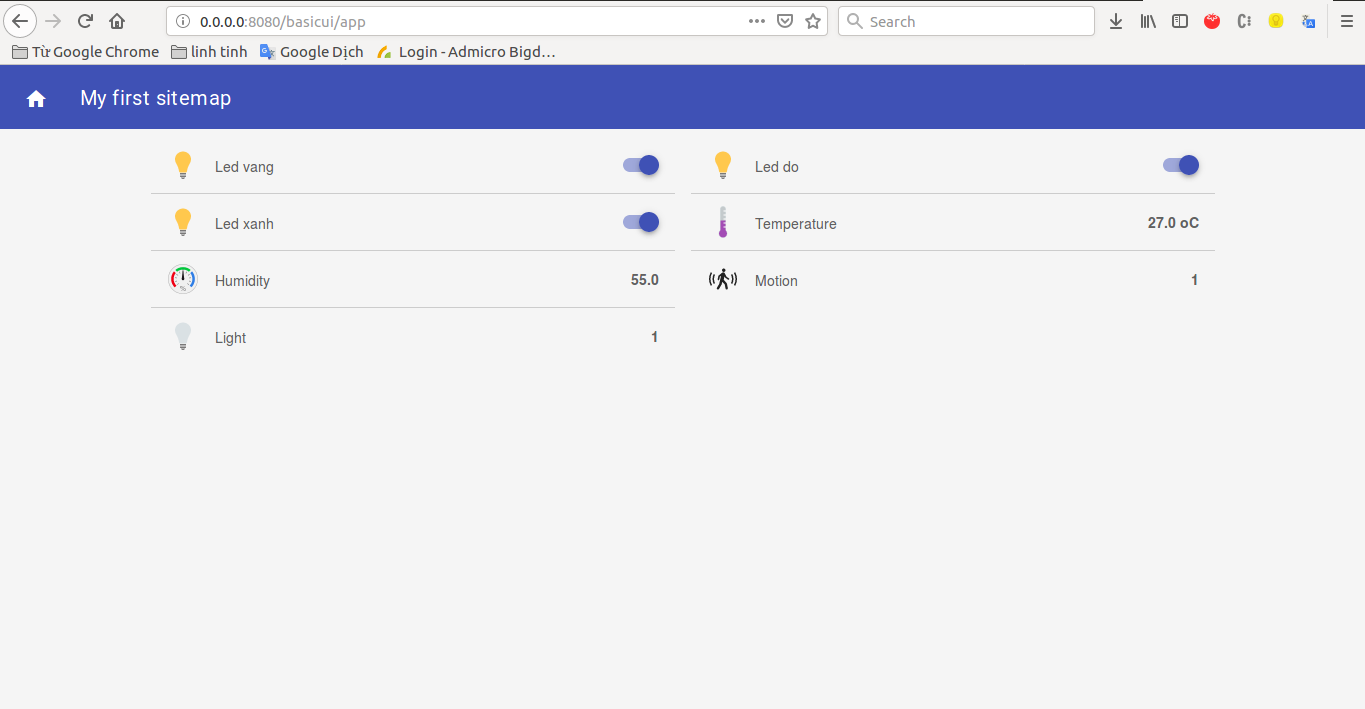
\includegraphics[scale=0.3]{image/openhab} \\
	\caption{Giao diện quản lý thiết bị của platform OpenHAB}
	\label{fig:giao_dien_openhab}
\end{figure}

Home Assistant là một nền tảng IoT mã nguồn mở ưu tiên quản lý các thiết bị trong ngôi nhà thông minh và có quan tâm tới tính riêng tư. Được cộng đồng lớn mạnh trên thế giới phát triển. Home Assistant phù hợp chạy trên Raspberry Pi hoặc một máy chủ tại chỗ. Home Assistant cũng lượng lớn hỗ trợ các thiết bị thông minh trên thị trường cũng như các giao thức phổ biến được sử dụng trong IoT. Giống với OpenHAB, Home Assistant cũng cung cấp các Restful API để lấy dữ liệu của thiết bị, đồng thời điều khiển các thiết bị qua các API này.
\clearpage

\begin{figure}[h!]
	\center
	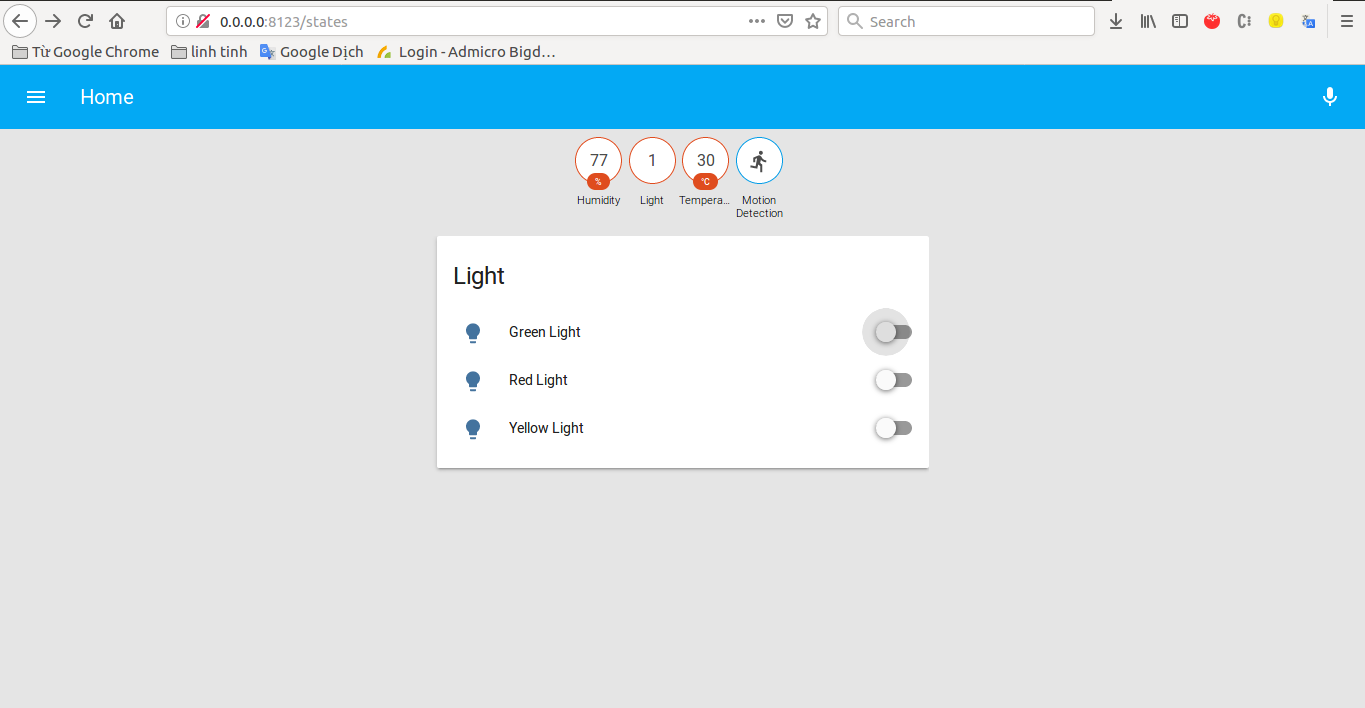
\includegraphics[scale=0.3]{image/homeassistant} \\
	\caption{Giao diện quản lý thiết bị của platform Home Assistant}
	\label{fig:giao_dien_homeassistant}
\end{figure}


Thingsboard là một nền tảng IoT mã nguồn mở giúp thu thập dữ liệu, xử lý,trực quan hóa dữ liệu và quản lý các thiết bị. Nó cho phép kết nối các thiết bị thông qua các giao thức chuẩn của IoT như MQTT, CoAp, HTTP. Thingsboard đảm bảo tính mở rộng, tính chịu lỗi và hiệu năng nên người dùng không sợ bị mất dữ liệu. Không giống như OpenHAB chưa có tính bảo mật dữ liệu, hay cơ chế bảo mật yếu Home Assistant, Thingsboard có cơ chế bảo mật dữ liệu của các thiết bị thông qua Token. Để truy cập được vào các thiết bị, bắt buộc phải biết token của các thiết bị này.

\begin{figure}[h!]
	\center
	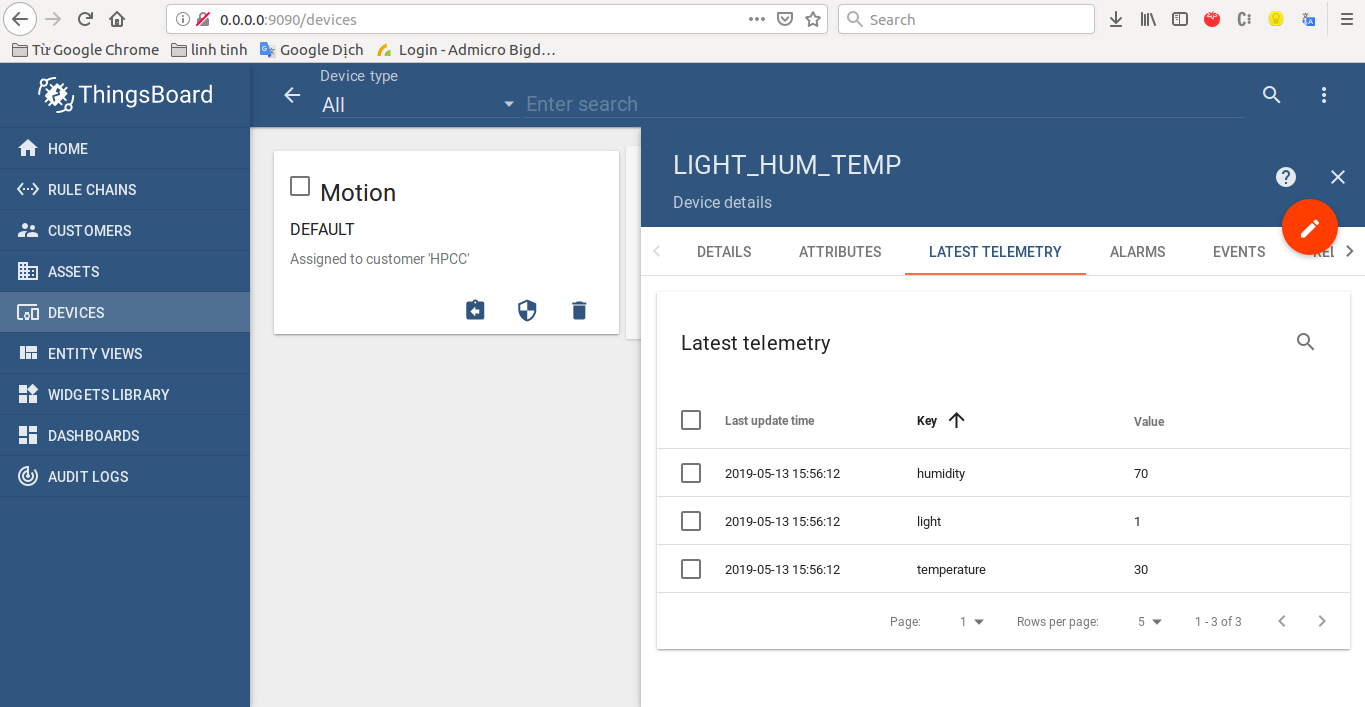
\includegraphics[scale=0.3]{image/thingsboard} \\
	\caption{Giao diện quản lý thiết bị của platform Thingsboard}
	\label{fig:giao_dien_thingsboard}
\end{figure}


\section{Xây dựng ontology}
Sau một thời gian làm việc, tôi đã xây dựng được một ontology như hình vẽ:

\clearpage
\begin{figure}[h!]
	\center
	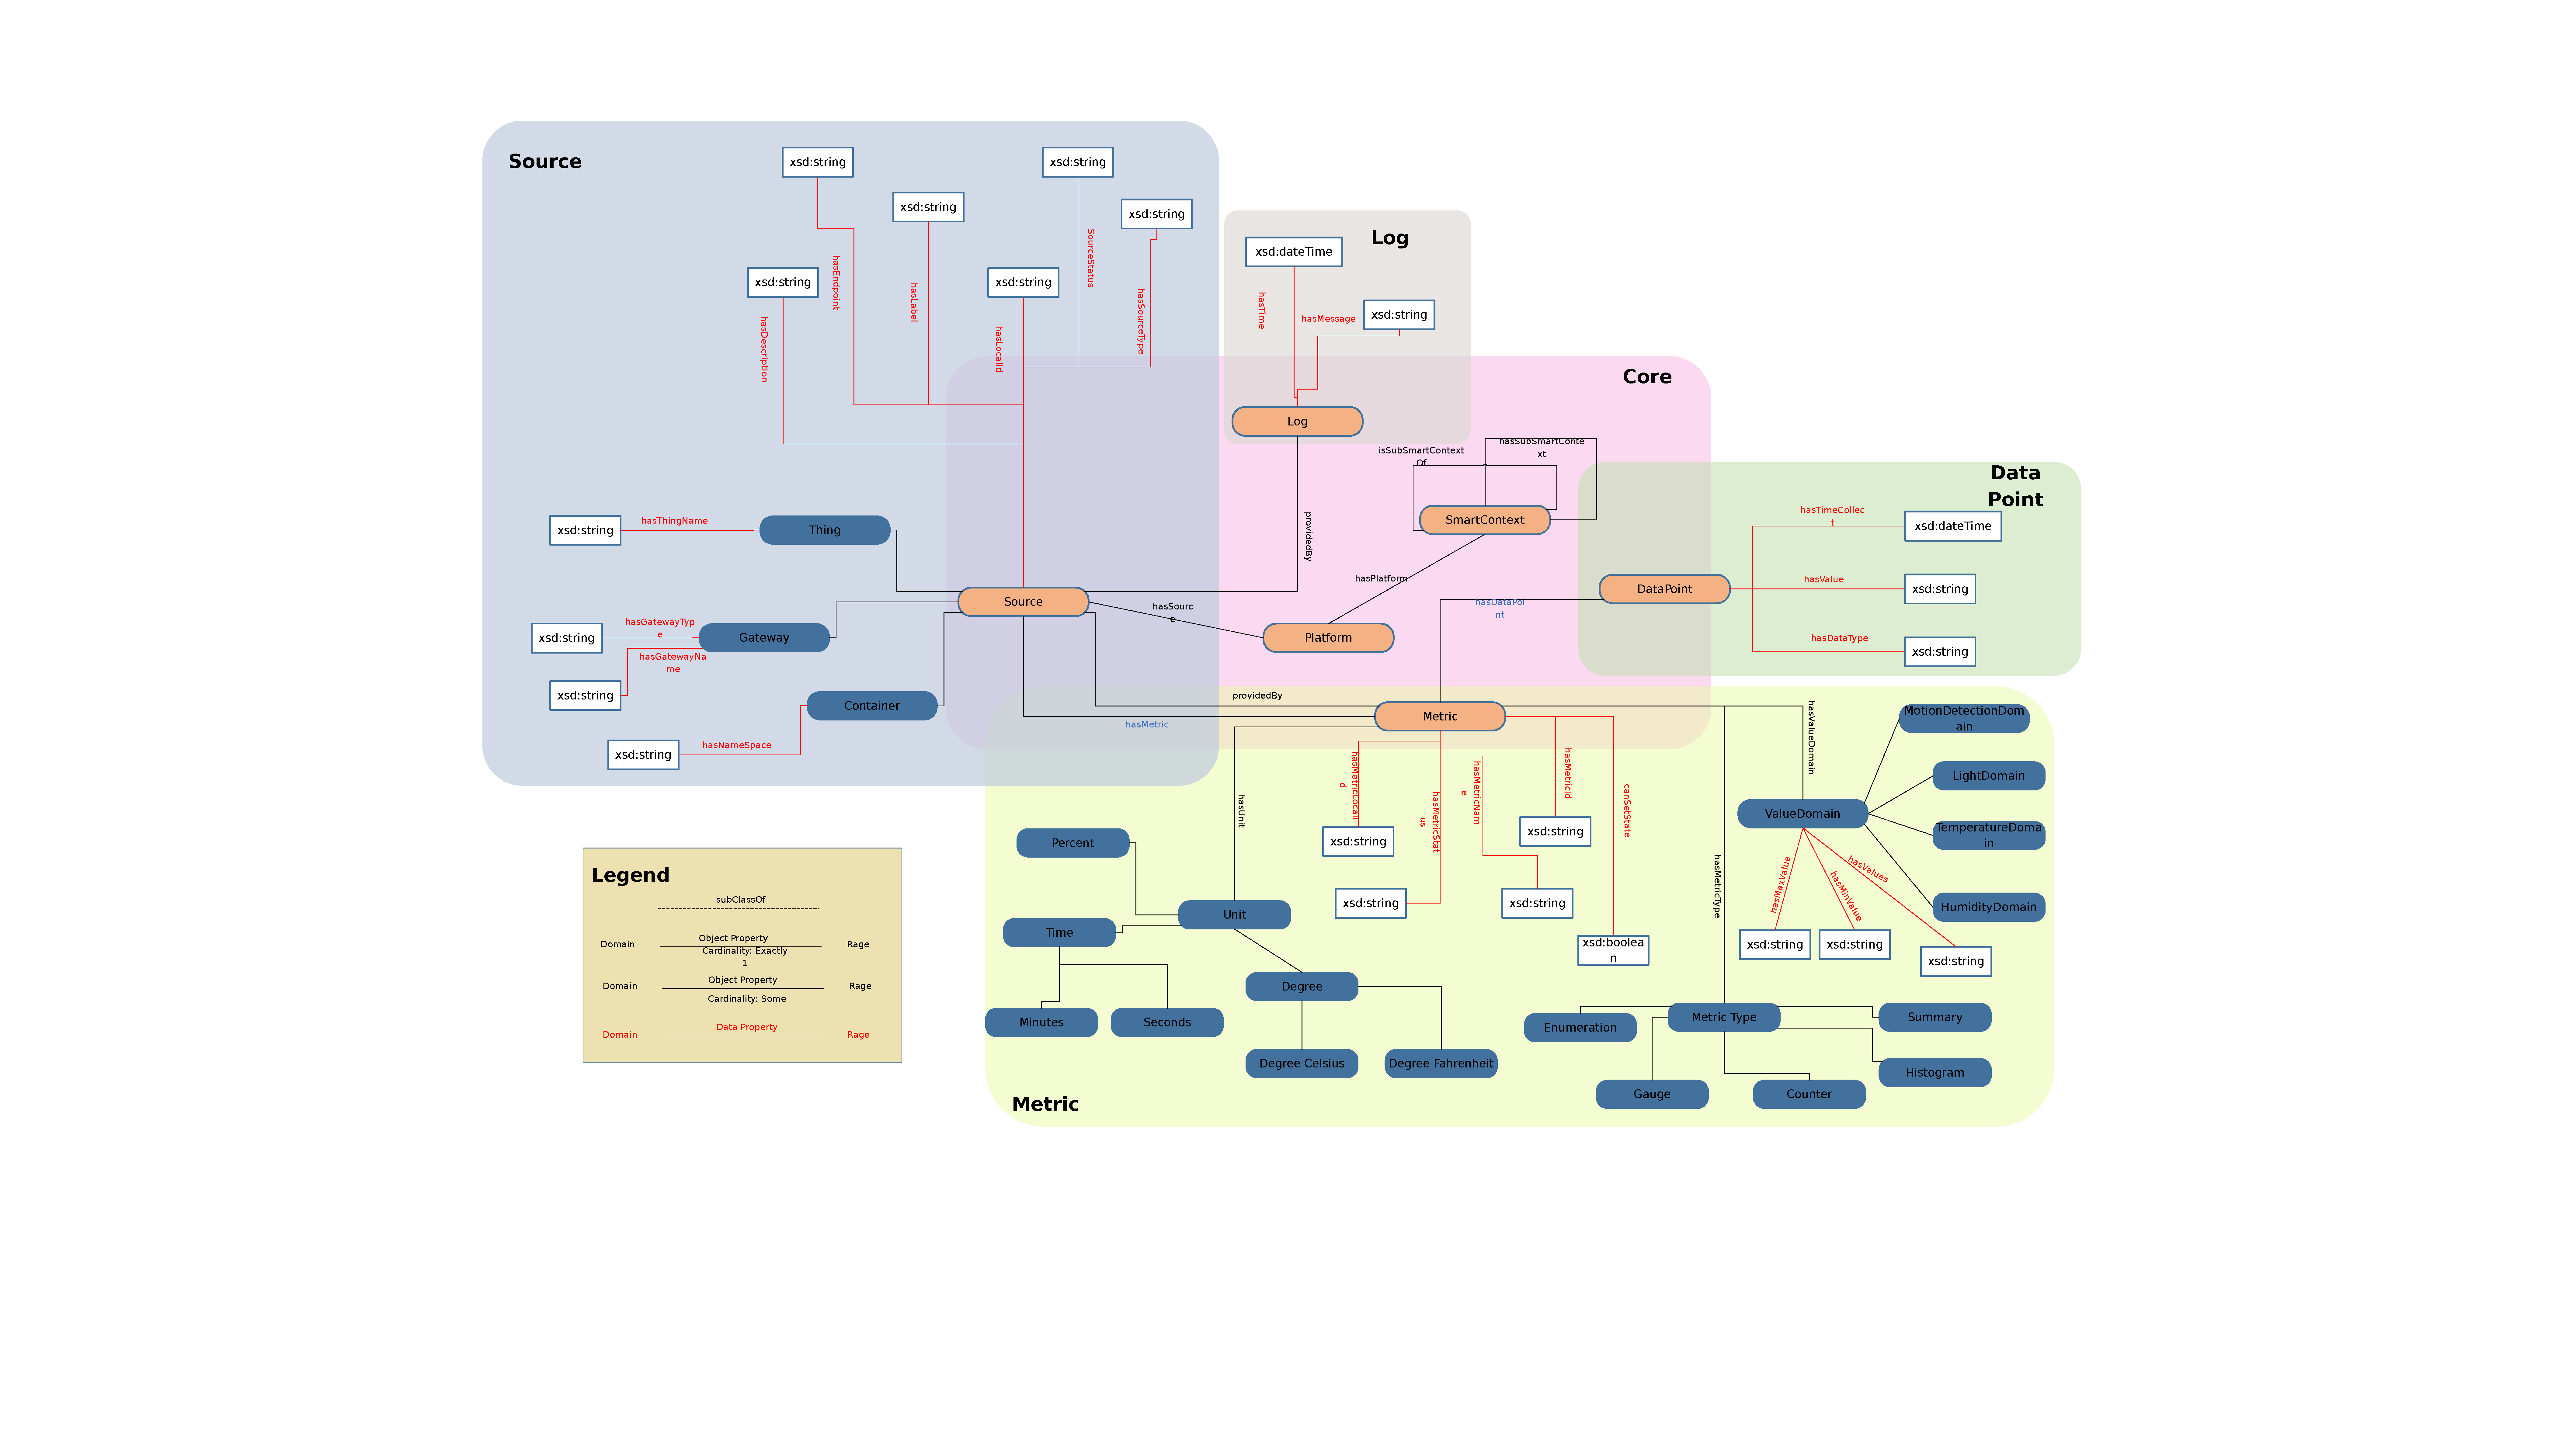
\includegraphics[scale=0.2, center]{image/ontology-2}
	\caption{ontology cho lĩnh vực nhà thông minh}
\end{figure}


Dưới đây là các bước xây dựng ontology mà tôi đã thực hiện:\\
\underline{Bước 1:} Xác định lĩnh vực và phạm vi của ontology \\
Lĩnh vực cần xây dựng ontology là IoT. Tuy nhiên, lĩnh vực IoT rất rộng lớn, gồm đa dạng các thiết bị, cảm biến và gồm nhiều khái niệm. Do đó, việc giới hạn phạm vi xây dựng ontology trong đề tài này là công việc quan trọng. Từ đó, tôi giới hạn phạm vi nghiên cứu của đề tài là lĩnh vực IoT trong nhà thông minh gồm có các thành phần: các cảm biến, các thiết bị, các nền tảng IoT, các ứng dụng/phạm vi sử dụng các nền tảng IoT. 
Mục đích sử dụng của ontology là để tạo ra các câu truy vấn ngữ nghĩa đơn giản. Một số câu hỏi ontology cần có thể trả lời được như:
\begin{itemize}
	\item Một khái niệm có những thuộc tính tương ứng nào?
	\item Một thực thể có các mối quan hệ với các thực thể nào khác?
	\item ...
\end{itemize}
Ngoài ra, ontology cũng cần có khả năng mở rộng so với các thành phần trong ngôi nhà thông minh. 

\underline{Bước 2:} Xem xét việc kế thừa các Ontology có sẵn: \\
Mặc dù đã tồn tại nhiều ontology như đã liệt kê trong chương 2, tuy nhiên, các ontology này chủ yếu được viết theo ngôn ngữ RDF, OWL dựa trên nền tảng web. Hơn nữa, các ontology này khá phức tạp, không phù hợp với phạm vi của đề tài. Do đó, tôi chỉ kế thừa các khái niệm, thuộc tính và các mối quan hệ trong các ontology này để xây dựng ontology của mình.

\underline{Bước 3:} Liệt kê các thuật ngữ quan trọng trong Ontology	\\
Một số khái niệm quan trọng trong lĩnh vực nhà thông minh: 
\begin{itemize}
	\item Smart Context: là một phạm vi triển khai hoặc một ứng dụng trong IoT. Đây sẽ là thành phần trên nhất trong cây phân cấp các khái niệm. Một smart context có thể chứa các smart context khác; một smart context cũng có thể nằm trong một smart context khác.
	\item Platform: là một phần mềm gồm nhiều thành phần, cho phép kết nối, quản lý và tự động hóa việc kết nối các thiết bị trong môi trường IoT. Nó kết nối các thiết bị phần cứng với nhau, cũng như với cloud bằng việc sử dụng linh hoạt các giao thức kết nối, cung cấp các cơ chế bảo mật và cung cấp năng lực xử lý dữ liệu.
	\item Source: Là một thiết bị vật lý hoặc thiết bị ảo. Source sẽ sinh ra dữ liệu về môi trường hay bất kỳ thứ gì mà nó theo dõi. Một Source có thể là một Thing, Gateway hay một Process Unit.
	\item Thing: Là một thiết bị, bao gồm một hoặc một tập hợp các cảm biến
	\item Gateway: Là một thiết bị vật lý hay một trình phần mềm phục vụ như là một điểm kết nối giữa các thiết bị thông minh, các cảm biến với cloud.
	\item Container: Là một thiết bị ảo để theo dõi các tài nguyên trong một hệ thống IoT như CPU, RAM, ổ đĩa, …
	\item Log: là dữ liệu được sinh ra từ Source. Các tệp tin log có thể được dùng để lấy ra các thông tin lịch sử của dữ liệu, trạng thái theo dõi các thiết bị, …
	\item Metric được sử dụng để nhấn mạnh các loại độ đo khác nhau của dữ liệu trong IoT.  Một số loại Metric có thể như Enumeration, Gauge, Counter, Histogram, Summary. Mỗi Metric có các đơn vị tương ứng như Percent, Time, Degree. Mỗi Source đều có một hoặc nhiều Metric của nó.
	\item Data Point: Được tạo ra khi một Source hoạt động. Dựa trên thông tin về Metric của một Source, dữ liệu sẽ có DataType, DataValue phù hợp.
\end{itemize}
\underline{Bước 4:} Xây dựng các lớp/khái niệm và cấu trúc lớp/khái niệm phân cấp: \\
Xây dựng theo kiểu trên xuống, ta nhận thấy Smart Context là khái niệm có mức độ tổng quát cao nhất, là gốc của đồ thị. Các khái niệm Log, Platform, Source, Metric, Data Point là các khái niệm trung gian. Các khái niệm Thing, Gateway, Container, Percent, Time, Degree, … là các khái niệm lá. 

\underline{Bước 5:} Định nghĩa các thuộc tính và quan hệ cho lớp:	\\
Các thuộc tính của các khái niệm trong ontology:
\hspace{0mm}Smart context có các thuộc tính:
\begin{itemize}
	\item SmartContextId: định danh duy nhất của một smart context
	\item SmartContextName: tên của một smartcontext
\end{itemize} 

\hspace{0mm}Platform có các thuộc tính:
\begin{itemize}
	\item PlatformId: định danh duy nhất của một platform
	\item PlatformName: tên của platform
	\item PlatformType: loại platform
	\item PlatformHost: địa chỉ của máy cài đặt platform này
	\item PlatformPort: Cổng cài đặt platform	
	\item PlatformStatus: trạng thái hoạt động của platform
\end{itemize}

\hspace{0mm}Source có các thuộc tính:
\begin{itemize}
	\item SourceId: Định danh toàn cục duy nhất của một Source
	\item EndPoint: Địa chỉ của Source
	\item SourceStatus: Trạng thái hoạt động của Source
	\item Description: Mô tả về Source
	\item SourceType: loại Source	
	\item Label: nhãn của Source
	\item LocalId: Địa chỉ cục bộ của Source
\end{itemize}



\hspace{0mm}Metric có các thuộc tính:
\begin{itemize}
	\item MetricId: định danh toàn cục duy nhất của một Metric
	\item MetricName: tên của một Metric
	\item MetricLocalId: định danh cục bộ của một Metric
	\item MetricType: loại Metric
	\item Unit: đơn vị của Metric
	\item ValueDomain: trường giá trị để ánh xạ các khác nhau trong việc biểu diễn các giá trị dữ liệu của cùng một thiết bị nhưng trong các platform khác nhau. Ví dụ, cùng một cảm biến nhiệt độ, nhưng OpenHAB biểu diễn giá trị của nó là 0/1, HomeAssistant biểu diễn giá trị là on/off.
\end{itemize}


\hspace{0mm}Data Point có các thuộc tính:
\begin{itemize}
	\item DataPointId: định danh duy nhất của một Data Point
	\item DataType: Kiểu dữ liệu của một Data Point
	\item time: thời điểm Data Point được thu nhận
	\item value: giá trị của Data Point
\end{itemize}


\hspace{0mm}Log có các thuộc tính:
\begin{itemize}
	\item time: thời điểm ghi log
	\item message: nội dung của log
\end{itemize}

\hspace{0mm}Mối quan hệ của các khái niệm:
\hspace{0mm}Smart Context
\begin{itemize}
	\item isSubSmartContext: smart context nằm trong smart context khác 
	\item hasSmartContextId: smart context chứa smart context khác.
	\item hasPlatform: smart context chứa platform nào.
\end{itemize}

\hspace{0mm}Platform:
\begin{itemize}
	\item hasSource: Platform chứa những Source nào
\end{itemize}

\hspace{0mm}Source:
\begin{itemize}
	\item hasMetric: Source chứa những Metric nào
\end{itemize}

\hspace{0mm}Metric:
\begin{itemize}
	\item hasDataPoint: Metric chứa những Data Point nào
\end{itemize}

\underline{Bước 6:} Định nghĩa các ràng buộc của các thuộc tính
\hspace{0mm}Các ràng buộc của các thuộc tính:
\hspace{0mm}Smart context: 
\begin{itemize}
	\item SmartContextId: phải là một kiểu String
	\item SmartContextName: phải là một kiểu String
\end{itemize}

\hspace{0mm}Platform:
\begin{itemize}
	\item PlatformId: phải là một kiểu String
	\item PlatformName: phải là một kiểu String
	\item PlatformType: phải là một kiểu String
	\item PlatformHost: phải là một kiểu String
	\item PlatformPort: phải là một kiểu String
	\item PlatformStatus: phải là một kiểu String
\end{itemize}


\hspace{0mm}Source:
\begin{itemize}
	\item SourceId: phải là một kiểu String
	\item EndPoint: phải là một kiểu String
	\item SourceStatus: phải là một kiểu String
	\item Description: phải là một kiểu String
	\item SourceType: phải là một kiểu String
	\item Label: phải là một kiểu String
	\item LocalId: phải là một kiểu String
\end{itemize}


\hspace{0mm}Metric:
\begin{itemize}
	\item MetricId: phải là một kiểu String
	\item MetricName: phải là một kiểu String
	\item MetricLocalId: phải là một kiểu String
	\item MetricType: phải là một kiểu String
	\item Unit: có thể là kiểu của Percent, Time hoặc Degree
	\item ValueDomain: phải là một kiểu String
\end{itemize}


\hspace{0mm}Data Point:
\begin{itemize}
	\item DataPointId: phải là một kiểu String
	\item DataType: phải là một kiểu String
	\item time: phải là một kiểu datetime
	\item value: phải là một kiểu Number
\end{itemize}


\hspace{0mm}Log có các thuộc tính:
\begin{itemize}
	\item time: phải là một kiểu datetime
	\item message: phải là một kiểu String
\end{itemize}


\underline{Bước 7:} Tạo ra các thực thể
Để tạo ra thực thể cho các khái niệm, tôi dùng cú pháp json thay thế cho cú pháp bộ ba: đối tượng - thuộc tính - giá trị với ý nghĩa tương đương.

\hspace{0mm}Một thực thể Smart context: \\
\clearpage
%\begin{figure}[h!]
%	\center
%	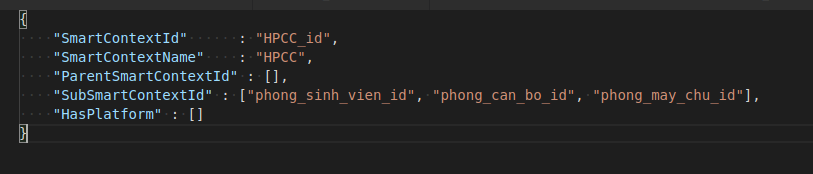
\includegraphics[scale=0.5]{image/smartcontext_instance}
%	\caption{Thực thể smartcontext}
%\end{figure}

\{\\
\blank{1cm}"SmartContextId" : "HPCC\_id", \\
\blank{1cm}"SmartContextName" : "HPCC",	\\
\blank{1cm}"ParentSmartContextId" : [],	\\
\blank{1cm}"SubSmartContextId" : ["phong\_sinh\_vien\_id", "phong\_can\_bo\_id", "phong\_may\_chu\_id"], \\
\blank{1cm}"HasPlatform" : []\\
\}



\hspace{0mm}Một thực thể Platform: \\
%\begin{figure}[h!]
%	\center
%	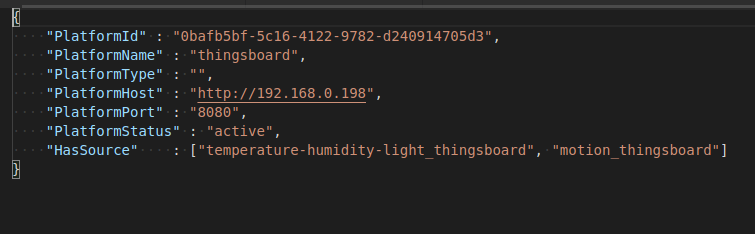
\includegraphics[scale=0.5]{image/platform_instance}
%	\caption{Thực thể platform}
%\end{figure}

\{\\
\blank{1cm}"PlatformId" : "611dc2c1-086d-487f-b44a-2d819764603a", \\
\blank{1cm}"PlatformName" : "homeassistant",	\\
\blank{1cm}"PlatformType" : "",	\\
\blank{1cm}"PlatformHost" : "http://192.168.0.199",\\
\blank{1cm}"PlatformPort" : "8123",\\
\blank{1cm}"PlatformStatus" : "active",\\
\blank{1cm}"HasSource" : ["temperature-humidity-light\_homeassistant", "motion\_homeassistant"]\\
\}

\hspace{0mm}Một thực thể Source:
%\begin{figure}[h!]
%	\center
%	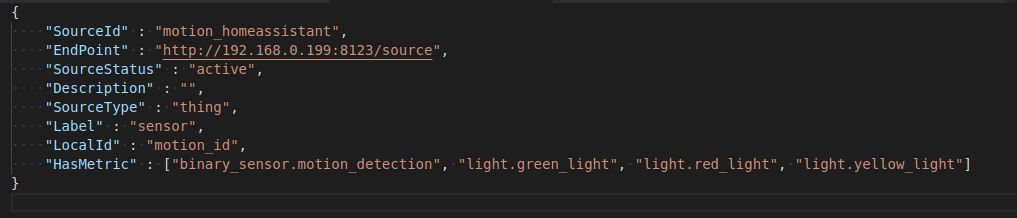
\includegraphics[scale=0.4]{image/source_instance}
%	\caption{Thực thể Source}
%\end{figure}

\{\\
\blank{1cm}"SourceId" : "motion\_homeassistant",\\
\blank{1cm}"EndPoint" : "http://192.168.0.199:8123/source",\\
\blank{1cm}"SourceStatus" : "active",\\
\blank{1cm}"Description" : "",\\
\blank{1cm}"SourceType" : "thing",\\
\blank{1cm}"Label" : "sensor",\\
\blank{1cm}"LocalId" : "motion\_id",\\
\blank{1cm}"HasMetric" : ["binary\_sensor.motion\_detection", "light.green\_light", "light.red\_light", "light.yellow\_light"] \\
\}

\hspace{0mm}Một thực thể Metric:
\clearpage
%\begin{figure}[h!]
%	\center
%	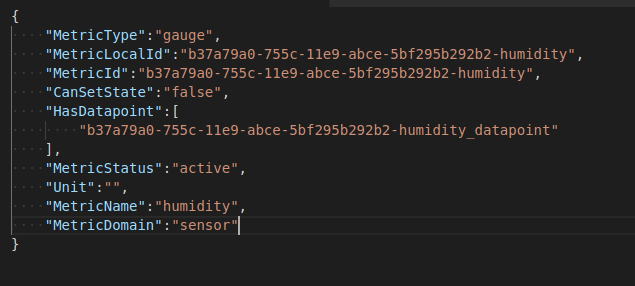
\includegraphics[scale=0.6]{image/metric_instance}
%	\caption{Thực thể Metric}
%\end{figure}

\{\\
\blank{1cm}"MetricType":"gauge",\\
\blank{1cm}"MetricLocalId":"b37a79a0-755c-11e9-abce-5bf295b292b2-humidity",\\
\blank{1cm}"MetricId":"b37a79a0-755c-11e9-abce-5bf295b292b2-humidity",\\
\blank{1cm}"CanSetState":"false",\\
\blank{1cm}"HasDatapoint":[
        "b37a79a0-755c-11e9-abce-5bf295b292b2-humidity\_datapoint"
    ],\\
\blank{1cm}"MetricStatus":"active",\\
\blank{1cm}"Unit":"",\\
\blank{1cm}"MetricName":"humidity",\\
\blank{1cm}"MetricDomain":"sensor"\\
\}

\hspace{0mm}Một thực thể Data Point:

%\begin{figure}[h!]
%	\center
%	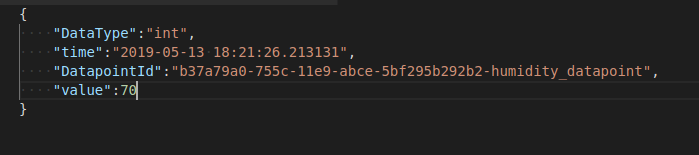
\includegraphics[scale=0.6]{image/datapoint_instance}
%	\caption{Thực thể Data Point}
%\end{figure}

\{\\
\blank{1cm}"DataType":"int",\\
\blank{1cm}"time":"2019-05-13 18:21:26.213131",\\
\blank{1cm}"DatapointId":"b37a79a0-755c-11e9-abce-5bf295b292b2-humidity\_datapoint"\\
\blank{1cm}"value":70\\
\}


\section{Xây dựng driver ánh xạ các dữ liệu trong IoT theo ontology}
Các dữ liệu từ các cảm biến, thiết bị IoT rất khác nhau về cấu trúc. Do trong đề tài này, tất cả các cảm biến, thiết bị đều được gắn với một platform; mỗi platform biểu diễn dữ liệu thu được từ các cảm biến, thiết bị theo một định dạng chuẩn riêng ta phải ánh xạ các định dạng dữ liệu chuẩn của các platform về một dạng chung. Để làm được điều này, ta phải viết các driver cho mỗi platform, nhiệm vụ của driver là ánh xạ định dạng dữ liệu của mỗi platform về định dạng dữ liệu chung của ontology. Để chứng minh khả năng mở rộng của hệ thống, tôi xây dựng driver cho hai nền tảng IoT là HomeAssistant và OpenHAB để ánh xạ định dạng dữ liệu của hai nền tảng này về định dạng của ontology. Sau đó, đến phần thực nghiệm khả năng mở rộng của hệ thống tôi sẽ thêm một nền tảng IoT khác là Thingsboard rồi tích hợp vào hệ thống bằng cách viết thêm một driver cho nền tảng này.\\
%Sau khi đã có một định dạng dữ liệu thống nhất, ta phải dùng ngôn ngữ hình thức để biểu diễn các khái niệm trong ontology. Ở đề tài này, tôi dùng định dạng json để biểu diễn các khái niệm, các thuộc tính của các khái niệm cũng như mối quan hệ giữa các khái niệm. 
%\clearpage
\begin{figure}[h!]
	\center
	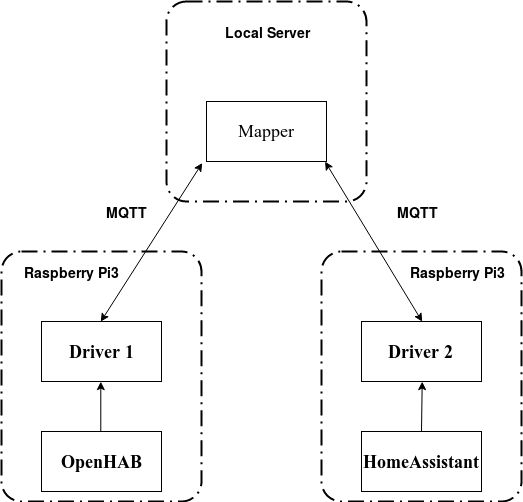
\includegraphics[scale=0.6]{image/mapping_service}
	\caption{Mô hình ánh xạ dữ liệu về một chuẩn của ontology}
\end{figure}


Định dạng dữ liệu của OpenHAB:

\begin{figure}[h!]
	\center
	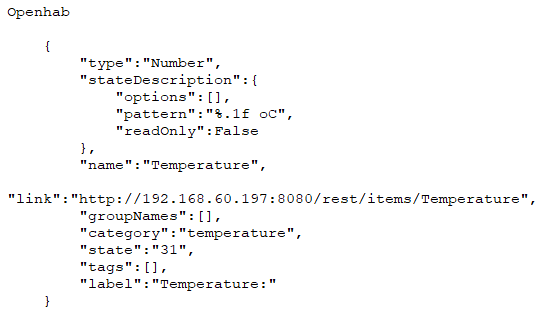
\includegraphics[scale=0.6]{image/openhab_dataformat}
	\caption{Định dạng dữ liệu của OpenHAB}
\end{figure}

Định dạng dữ liệu của HomeAssistant
\clearpage
\begin{figure}[h!]
	\center
	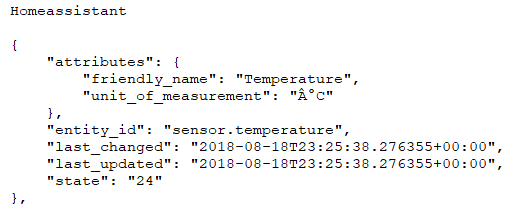
\includegraphics[scale=0.6]{image/homeassistant_dataformat}
	\caption{Định dạng dữ liệu của HomeAssistant}
\end{figure}

Sau khi qua thành phần ánh xạ, dữ liệu của hai nền tảng IoT sẽ được chuẩn hóa về định dạng của ontology.
%Định dạng dữ liệu của ontology:
%\begin{figure}[h!]
%	\center
%	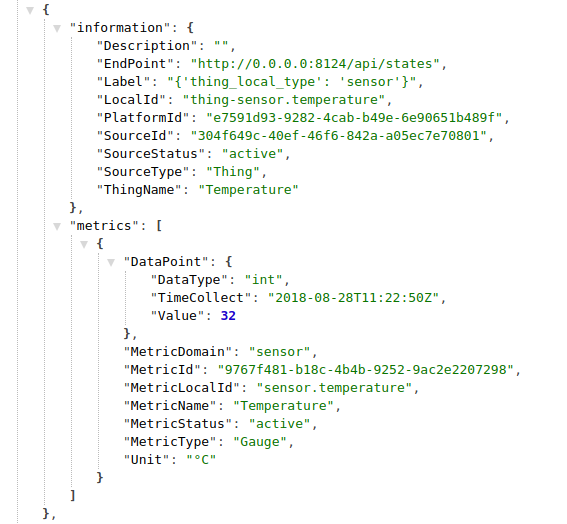
\includegraphics[scale=0.6]{image/ontology_dataformat}
%	\caption{Định dạng dữ liệu của Ontology}
%\end{figure}

\section{Xây dựng cơ chế truy vấn ngữ nghĩa}

\subsection{Cơ chế truy vấn ngữ nghĩa}
Từ các thực thể được biểu diễn theo ontology, ta phải xây dựng cơ chế để lấy được thông tin của các thực thể, mối quan hệ giữa các thực thể. Để làm được điều này, tôi xây dựng tập các API dựa vào mối quan hệ giữa các khái niệm để đạt được tính ngữ nghĩa. Đồng thời, tôi định nghĩa một ngôn ngữ truy vấn đơn giản, sử dụng tập API trên để tạo ra các câu truy vấn ngữ nghĩa.

Nhánh query của một statement tương ứng với việc thực hiện một câu truy vấn ngữ nghĩa. Để thực hiện câu truy vấn, ta cần chỉ rõ muốn lấy thuộc tính hay khái niệm nào, tập các thuộc tính và khái niệm được gọi là keyword. Ngoài việc chỉ rõ các thuộc tính, khái niệm cần truy vấn, ta cũng cần chỉ rõ điều kiện thực hiện câu truy vấn. Điều kiện này được chứa trong thành phần "Condition". Một chức năng khác mà ta mong muốn có thể thực hiện là kiểm tra các điều kiện, nếu điều kiện thỏa mãn thì thực hiện một hành động nào đó, hành động này tương ứng với việc điều khiển các thiết bị IoT dựa trên các API mà các platform cung cấp. Chức năng này được gọi là rule. Các thành phần của một câu truy vấn:


\begin{figure}[h!]
	\center
	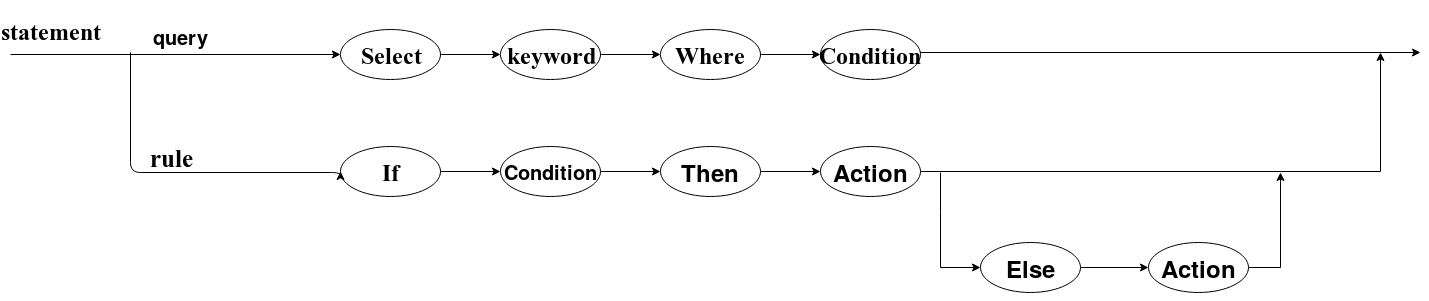
\includegraphics[scale=0.3]{image/language_model-statement}
	\caption{Mô hình ngôn ngữ - statement}
\end{figure}


Một condition là một phép so sánh giữa giá trị tương ứng một keyword với một biểu thức. Ví dụ so sánh PlatformId = "OpenHAB\_id". Các phép so sánh có thể có là <, >, >=, <=, =, !=. Tùy thuộc vào keyword mà có phép so sánh tương ứng. Condition cũng có thể là kết quả của một phép toán logic của một tập hợp các condition khác. Hai phép toán logic hỗ trợ là AND và OR. Ngoài ra, để thể hiện thứ tự ưu tiên của các phép toán logic, ta đưa thêm cặp dấu ngoặc đơn vào ngôn ngữ.

\begin{figure}[h!]
	\center
	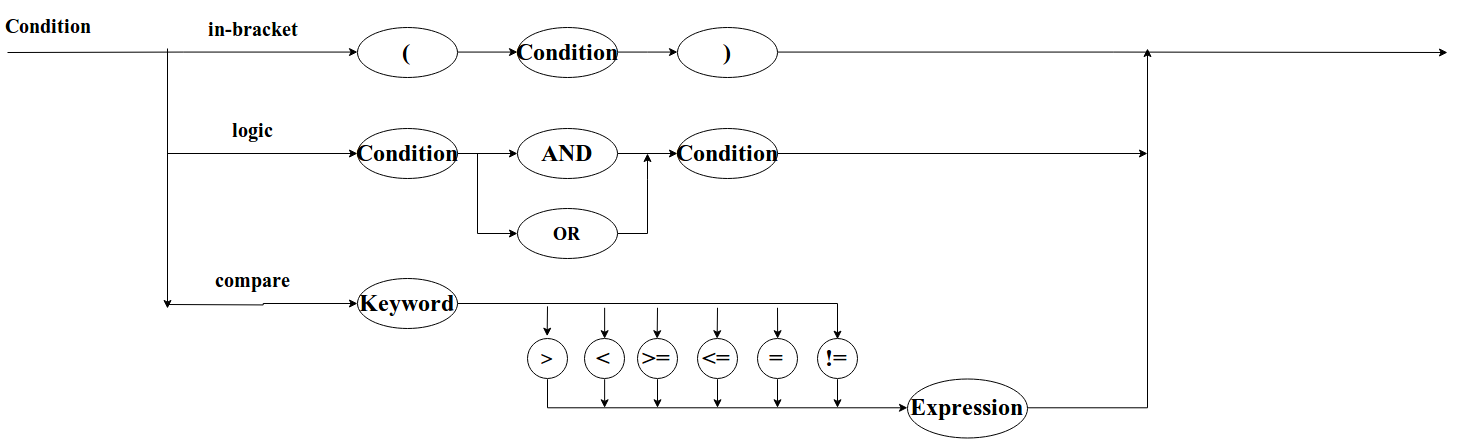
\includegraphics[scale=0.3]{image/language_model-condition}
	\caption{Mô hình ngôn ngữ - condition}
\end{figure}


Một Action (hành động) là một lời gọi tới các API để điều khiển các thiết bị từ nền tảng IoT. Do các thiết bị trong hệ thống chỉ cung cấp hai thao tác điều khiển là bật và tắt nên ngôn ngữ chỉ đưa vào hai hành động là bật và tắt.

\begin{figure}[h!]
	\center
	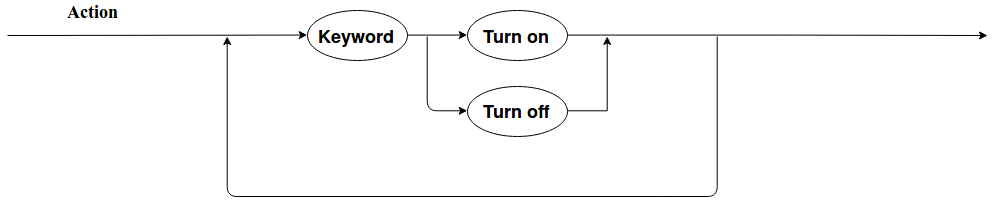
\includegraphics[scale=0.4]{image/language_model-action}
	\caption{Mô hình ngôn ngữ - action}
\end{figure}


Một biểu thức là một toán tử hoặc các phép toán cộng, trừ các toán tử.
\begin{figure}[h!]
	\center
	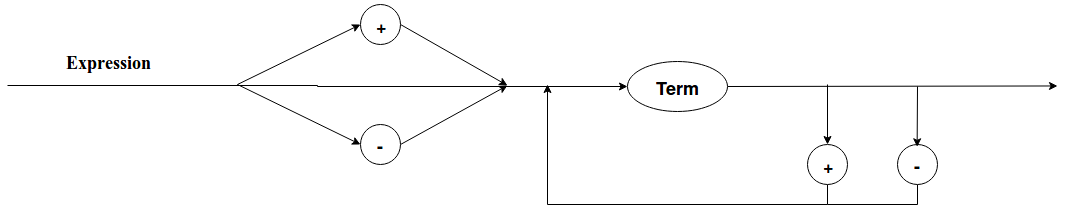
\includegraphics[scale=0.4]{image/language_model-expression}
	\caption{Mô hình ngôn ngữ - expression}
\end{figure}

Một toán tử là một hằng số hoặc các phép toán của các hằng số.
\begin{figure}[h!]
	\center
	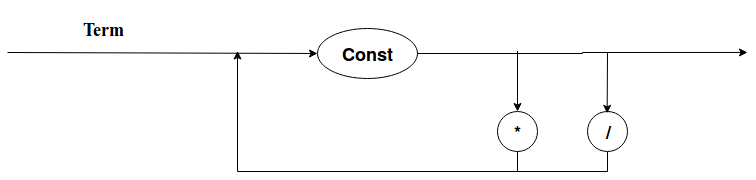
\includegraphics[scale=0.4]{image/language_model-term}
	\caption{Mô hình ngôn ngữ - term}
\end{figure}

Một hằng số là một chuỗi hoặc một số (nguyên hoặc thực).
\begin{figure}[h!]
	\center
	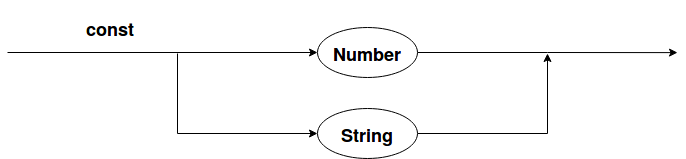
\includegraphics[scale=0.4]{image/language_model-const}	
	\caption{Mô hình ngôn ngữ -const}
\end{figure}
\clearpage


\subsection{Biểu đồ use case tổng quát}

\begin{figure}[h!]
	\center
	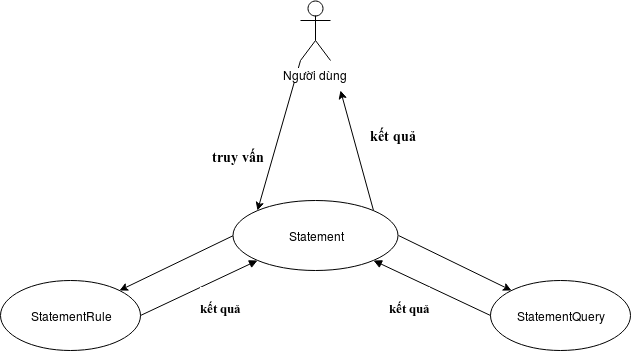
\includegraphics[scale=0.6]{image/language_diagram-use_case}
	\caption{Biểu đồ use case tổng quát}
\end{figure}


\subsection{Biểu đồ lớp của các thành phần của cơ chế truy vấn}

\begin{figure}[h!]
	\center
	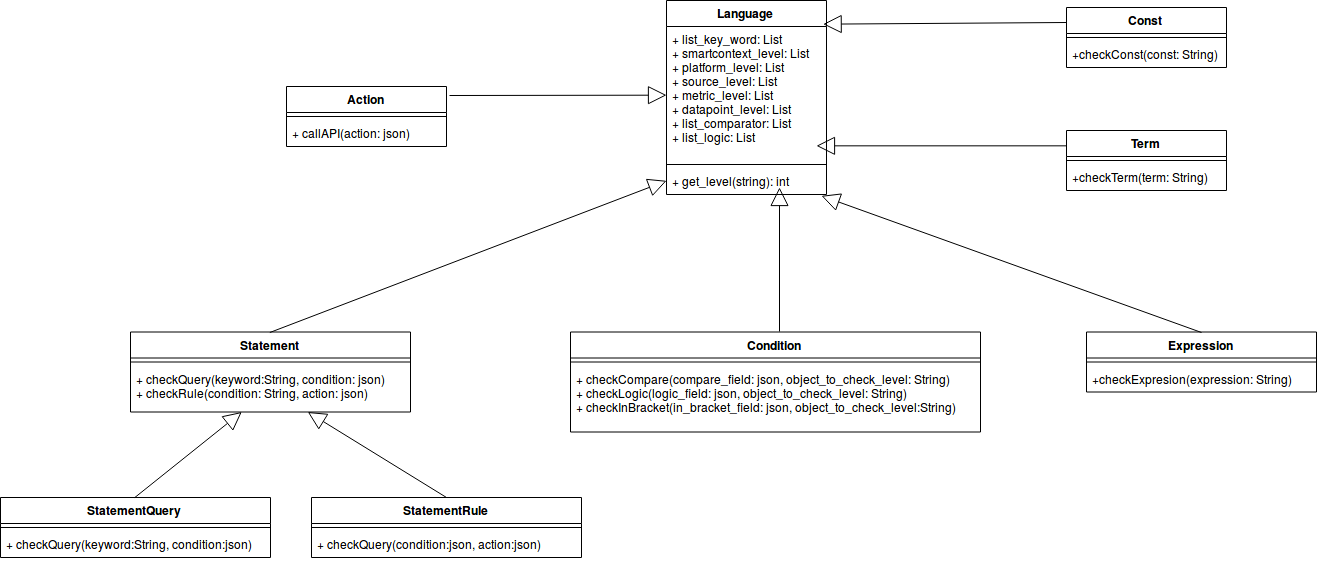
\includegraphics[scale=0.35]{image/language_diagram-class_diagram}	
	\caption{Biểu đồ lớp của các thành phần}
\end{figure}


\subsection{Biểu đồ hoạt động các thành phần của cơ chế truy vấn}

\begin{figure}[h!]
	\center
	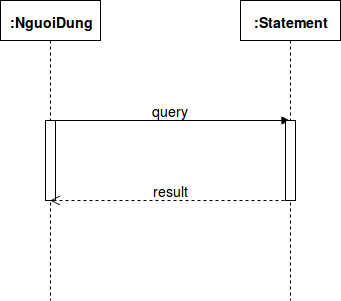
\includegraphics[scale=0.4]{image/language_diagram-statement}	
	\caption{Biểu đồ hoạt động của thành phần Statement}
\end{figure}


\begin{figure}[h!]
	\center
	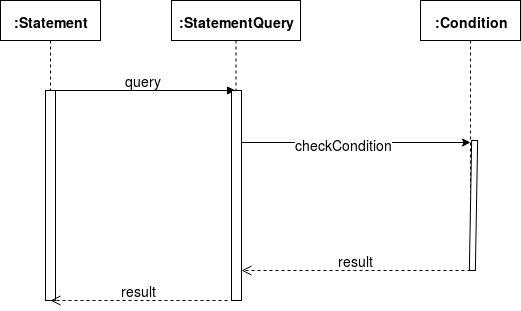
\includegraphics[scale=0.4]{image/language_diagram-statement_query}	
	\caption{Biểu đồ hoạt động của thành phần StatementQuery}
\end{figure}


\begin{figure}[h!]
	\center
	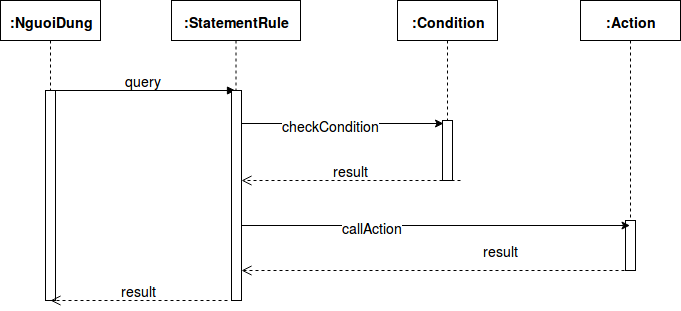
\includegraphics[scale=0.4]{image/language_diagram-statement_rule}	
	\caption{Biểu đồ hoạt động của thành phần StatementRule}
\end{figure}


\begin{figure}[h!]
	\center
	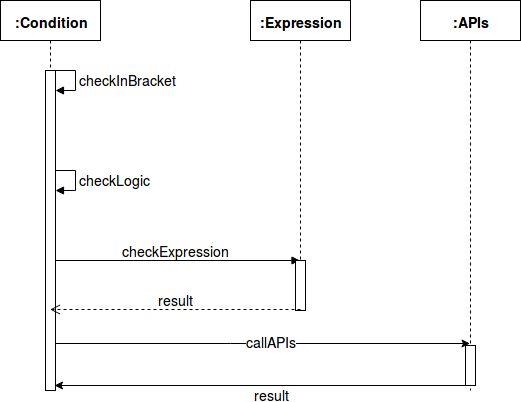
\includegraphics[scale=0.4]{image/language_diagram-condition}	
	\caption{Biểu đồ hoạt động của thành phần Condition}
\end{figure}


\begin{figure}[h!]
	\center
	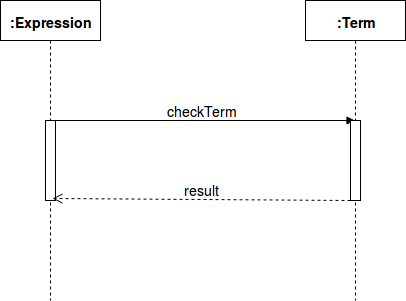
\includegraphics[scale=0.4]{image/language_diagram-expression}	
	\caption{Biểu đồ hoạt động của thành phần Expression}
\end{figure}


\begin{figure}[h!]
	\center
	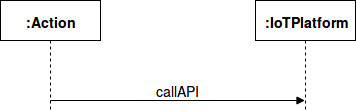
\includegraphics[scale=0.4]{image/language_diagram-action}	
	\caption{Biểu đồ hoạt động của thành phần Action}
\end{figure}


\begin{figure}[h!]
	\center
	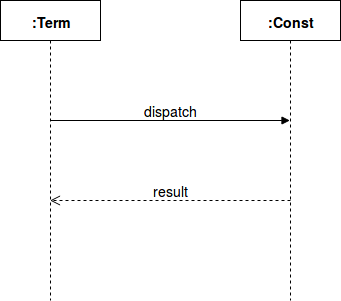
\includegraphics[scale=0.4]{image/language_diagram-term}	
	\caption{Biểu đồ hoạt động của thành phần Term}
\end{figure}


\subsection{Tập các API}
Để cài đặt cơ chế ngữ nghĩa, tôi đã xây dựng tập các API, các API này dựa vào mối quan hệ giữa các khái niệm trong ontology để thực hiện các câu truy vấn ngữ nghĩa. \\

Các API cơ bản:

\begin{itemize}
	\item Lấy tất cả các Data Point
	\item Lấy tất cả các Metric
	\item Lấy tất cả các Source
	\item Lấy tất cả các Platform
	\item Lấy tất cả các Smart Context
	\item Lấy tất cả các Smart Context nằm trong Smart Context nào đó. (lấy smart context con)
	\item Lấy tất cả các Smart Context chứa Smart Context nào đó. (lấy smart context cha)
\end{itemize}

Một số API phụ trợ:
\begin{itemize}
	\item Lấy DataPointId/DataPoint của một DataPoint
	\item Lấy MetricId/Metric của một Metric
	\item Lấy SourceId/Source của một Source
	\item Lấy PlatformId/Platform của một Platform
	\item Lấy SmartContextId/SmartContext của một SmartContext
\end{itemize}


Các API thể hiện tính ngữ nghĩa dựa trên mối quan hệ giữa các khái niệm:
\begin{itemize}
	\item Lấy DataPoint từ một Metric
	\item Lấy DataPoint từ một Source
	\item Lấy DataPoint từ một Platform
	\item Lấy DataPoint từ một SmartContext
	\item Lấy Metric từ một DataPoint
	\item Lấy Metric từ một Source
	\item Lấy Metric từ một Platform
	\item Lấy Metric từ một SmartContext
	\item Lấy Source từ một DataPoint
	\item Lấy Source từ một Metric
	\item Lấy Source từ một Platform
	\item Lấy Source từ một SmartContext
	\item Lấy Platform từ một DataPoint
	\item Lấy Platform từ một Metric
	\item Lấy Platform từ một Source
	\item Lấy Platform từ một SmartContext
	\item Lấy SmartContext từ một DataPoint
	\item Lấy SmartContext từ một Metric
	\item Lấy SmartContext từ một Source
	\item Lấy SmartContext từ một Platform
\end{itemize}


Ví dụ về cơ chế ngữ nghĩa trong API: Lấy DataPoint từ một SmartContext.
Các bước để lấy DataPoint từ SmartContext:
\begin{enumerate}
	\item lấy ra các Platform mà Smart Context đó chứa dựa vào mối quan hệ hasPlatform của SmartContext.
	\item với mỗi Platform, xác định xem nó chứa các Source nào dựa vào mối quan hệ hasSource của Platform.
	\item với mỗi Source, xác định xem nó chứa các Metric nào dựa vào mối quan hệ hasMetric của Source.
	\item với mỗi Metric, xác định DataPoint mà nó chứa dựa vào thuộc tính hasDataPoint của Metric.
\end{enumerate}

Vậy sau khi duyệt qua các quan hệ trên ontology, ta sẽ lấy ra được các DataPoint nằm trong một SmartContext. Cơ chế truy vấn ngữ nghĩa này hoàn toàn tương tự đối với các API khác được xây dựng.
\chapter{Thử nghiệm hệ thống}
\renewcommand{\baselinestretch}{1.2}
%\newcommand{\blank}[1]{\hspace*{#1}\linebreak[0]}
\section{Thử nghiệm tính ngữ nghĩa của câu truy vấn}
Để chứng minh tính đúng đắn của hệ thống, tôi thực hiện thử nghiệm hệ thống với một câu truy vấn: Liệt kê các thiết bị trong trung tâm HPCC. \\
Câu truy vấn tương ứng trong hệ thống của tôi là:
\myexample{Câu truy vấn tương ứng trong hệ thống}{
\{\\
\blank{1cm}"select" : "Source",\\
\blank{1cm}"where" : \{\\
\blank{2cm}"condition" : \{\\
\blank{3cm}"compare" : \{\\
\blank{4cm}    "keyword" : "SmartContextName",\\
\blank{4cm}    "comparator" : "=",\\
\blank{4cm}    "expression" : "HPCC"\\
\blank{3cm}\},\\
\blank{3cm}"logic" : \{\},\\
\blank{3cm}"in\_bracket" : \{\}\\
\blank{2cm}\}\\
\blank{1cm}\}\\
\}
}

Cơ chế truy vấn ngữ nghĩa: \\
\begin{figure}
	\center
	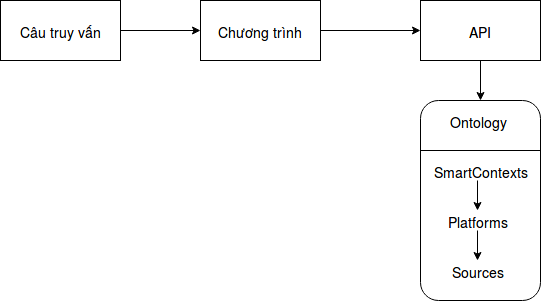
\includegraphics[scale=0.6]{image/demo}
	\caption{Cơ chế truy vấn ngữ nghĩa}
\end{figure}
Khi nhận được một câu truy vấn, hệ thống sẽ kiểm tra cú pháp câu truy vấn đó. Nếu cú pháp chính xác, sẽ gọi các API để trả về kết quả. Các API được xây dựng dựa trên mối quan hệ giữa các khái niệm trong ontology. Cụ thể trong trường hợp này, để trả về kết quả câu truy vấn, ta cần thực hiện các bước sau: \\
Đầu tiên, hệ thống sẽ tìm các SmartContext có tên là HPCC, kết quả thu được: \\
\myexample{}{
[\\
\blank{1cm}\{\\
\blank{2cm}'HasPlatform':[ ],\\
\blank{2cm}'ParentSmartContextId':[\\
\blank{3cm}'phong\_sinh\_vien\_id', \\
\blank{3cm}'phong\_can\_bo\_id', \\
\blank{3cm}'phong\_may\_chu\_id'\\
\blank{2cm}],\\
\blank{2cm}'SubSmartContextId':[ ],\\
\blank{2cm}'SmartContextId':'HPCC\_id',\\
\blank{2cm}'SmartContextName':'HPCC'\\
\blank{1cm}\}\\
]
}

Với mỗi SmartContext thu được, liệt kê các platform có trong đó: \\

\myexample{}{
[\\
\blank{1cm}\{\\
\blank{2cm}'PlatformHost':'http://192.168.0.197',\\
\blank{2cm}'PlatformId':'2667a8d0-0ff1-4d22-9153-26795502efc9',\\
\blank{2cm}'PlatformType':'',\\
\blank{2cm}'PlatformName':'openhab',\\
\blank{2cm}'PlatformPort':'8080',\\
\blank{2cm}'HasSource':[\\
\blank{3cm}'temperature-humidity-light\_openhab',\\
\blank{3cm}'motion\_openhab'\\
\blank{2cm}],\\
\blank{2cm}'PlatformStatus':'active'\\
\blank{1cm}\},\\
\blank{1cm}\{\\
\blank{2cm}'PlatformHost':'http://192.168.0.198',\\
\blank{2cm}'PlatformId':'0bafb5bf-5c16-4122-9782-d240914705d3',\\
\blank{2cm}'PlatformType':'',\\
\blank{2cm}'PlatformName':'thingsboard',\\
\blank{2cm}'PlatformPort':'8080',\\
\blank{2cm}'HasSource':[\\
\blank{3cm}'temperature-humidity-light\_thingsboard',\\
\blank{3cm}'motion\_thingsboard'\\
\blank{2cm}],\\
\blank{2cm}'PlatformStatus':'active'\\
\blank{1cm}\},
}
\myexample{}{
\blank{1cm}\{\\
\blank{2cm}'PlatformHost':'http://192.168.0.199',\\
\blank{2cm}'PlatformId':'611dc2c1-086d-487f-b44a-2d819764603a',\\
\blank{2cm}'PlatformType':'HomeAssistant',\\
\blank{2cm}'PlatformName':'homeassistant',\\
%}
%\myexample{}{
\blank{2cm}'PlatformPort':'8123',\\
\blank{2cm}'HasSource':[\\
\blank{3cm}'temperature-humidity-light\_homeassistant',\\
\blank{3cm}'motion\_homeassistant'\\
\blank{2cm}],\\
\blank{2cm}'PlatformStatus':'active'\\
\blank{1cm}\}\\
]
}

Ứng với mỗi platform, tìm các Soruce của mỗi platform. Ví dụ với platform OpenHAB:\\
\myexample{}{
[\\
\blank{1cm}\{\\
\blank{2cm}'LocalId':'temperature-humidity-light\_id',\\
\blank{2cm}'Label':'sensor',\\
\blank{2cm}'Description':'',\\
\blank{2cm}'SourceId':'temperature-humidity-light\_openhab',\\
\blank{2cm}'HasMetric':[\\
\blank{3cm}'Humidity',\\
\blank{3cm}'Temperature',\\
\blank{3cm}'Light'\\
\blank{2cm}],\\
\blank{2cm}'SourceType':'thing',\\
\blank{2cm}'SourceStatus':'active',
}
\myexample{}{
\blank{2cm}'EndPoint':'http://192.168.0.197:8080/source'\\
\blank{1cm}\},\\
\blank{1cm}\{\\
\blank{2cm}'LocalId':'motion\_id',\\
\blank{2cm}'Label':'sensor',\\
\blank{2cm}'Description':'',\\
\blank{2cm}'SourceId':'motion\_openhab',\\
\blank{2cm}'HasMetric':[\\
\blank{3cm}'LedDo',\\
\blank{3cm}'LedXanh',\\
\blank{3cm}'LedVang',\\
\blank{3cm}'Motion'\\
\blank{2cm}],\\
\blank{2cm}'SourceType':'thing',\\
\blank{2cm}'SourceStatus':'active',\\
\blank{2cm}'EndPoint':'http://192.168.0.197:8080/source'\\
\blank{1cm}\}\\
]
}

Kết quả cuối cùng thu được các Source của một SmartContext: \\

\myexample{}{
[\\
\blank{1cm}\{\\
\blank{2cm}'LocalId':'temperature-humidity-light\_id',\\
\blank{2cm}'SourceStatus':'active',\\
\blank{2cm}'Description':'',\\
\blank{2cm}'EndPoint':'http://192.168.0.197:8080/source',\\
\blank{2cm}'SourceId':'temperature-humidity-light\_openhab',
}
\myexample{}{
\blank{2cm}'HasMetric':[\\
\blank{3cm}'Humidity',\\
\blank{3cm}'Temperature',\\
\blank{3cm}'Light'\\
\blank{2cm}],\\
\blank{2cm}'SourceType':'thing',\\
\blank{2cm}'Label':'sensor'\\
\blank{1cm}\},\\
\blank{1cm}\{\\
\blank{2cm}'LocalId':'motion\_id',\\
\blank{2cm}'SourceStatus':'active',\\
\blank{2cm}'Description':'',\\
\blank{2cm}'EndPoint':'http://192.168.0.197:8080/source',\\
\blank{2cm}'SourceId':'motion\_openhab',\\
\blank{2cm}'HasMetric':[\\
\blank{3cm}'LedDo',\\
\blank{3cm}'LedXanh',\\
\blank{3cm}'LedVang',\\
\blank{3cm}'Motion'\\
\blank{2cm}],\\
\blank{2cm}'SourceType':'thing',\\
\blank{2cm}'Label':'sensor'\\
\blank{1cm}\},\\
\blank{1cm}\{\\
\blank{2cm}'LocalId':'temperature-humidity-light\_id',\\
\blank{2cm}'SourceStatus':'active',\\
\blank{2cm}'Description':'',\\
\blank{2cm}'EndPoint':'http://192.168.0.198:8080/source',\\
\blank{2cm}'SourceId':'temperature-humidity-light\_thingsboard',
}
\myexample{}{
\blank{2cm}'HasMetric':[\\
\blank{3cm}'b37a79a0-755c-11e9-abce-5bf295b292b2-light',\\
\blank{3cm}'b37a79a0-755c-11e9-abce-5bf295b292b2-temperature',\\
\blank{3cm}'b37a79a0-755c-11e9-abce-5bf295b292b2-humidity'\\
\blank{2cm}],\\
\blank{2cm}'SourceType':'thing',\\
\blank{2cm}'Label':'sensor'\\
\blank{1cm}\},\\
\blank{2cm}...\\
]
}
\clearpage

\section{Thử nghiệm tính mở rộng của hệ thống}
Để chứng minh hệ thống có tính khả mở, tôi thêm một nền tảng IoT là ThingsBoard vào hệ thống bằng việc viết thêm một driver để ánh xạ dữ liệu từ định dạng của ThingsBoard về định dạng của ontology. Tôi sẽ thực hiện câu truy vấn: Lấy tất cả các platform có trong trung tâm HPCC để chứng minh đã thêm được ThingsBoard vào hệ thống. \\
Câu truy vấn tương ứng trong hệ thống là:
%\begin{figure}
%	\center
%	\includegraphics[scale=0.5]{image/add_thingsboard}
%	\caption{Thêm ThingsBoard vào hệ thống}
%\end{figure}
\myexample{Câu truy vấn tương ứng trong hệ thống}{
\{\\
\blank{1cm}"select" : "Platform",\\
\blank{1cm}"where" : \{\\
\blank{2cm}"condition" : \{\\
\blank{3cm}"compare" : \{\\
\blank{4cm}    "keyword" : "SmartContextName",\\
\blank{4cm}    "comparator" : "=",\\
\blank{4cm}    "expression" : "HPCC"\\
\blank{3cm}\},\\
\blank{3cm}"logic" : \{\},\\
\blank{3cm}"in\_bracket" : \{\}\\
\blank{2cm}\}\\
\blank{1cm}\}\\
\}\\
}

\clearpage
Kết quả thu được trước khi thêm Thingsboard, hệ thống chỉ có 2 nền tảng IoT: \\

\myexample{}{
[\\
\blank{1cm}\{\\
\blank{2cm}'PlatformId':'2667a8d0-0ff1-4d22-9153-26795502efc9',\\
\blank{2cm}'PlatformHost':'http://192.168.0.197',\\
\blank{2cm}'PlatformName':'openhab',\\
\blank{2cm}'HasSource':[\\
\blank{3cm}'temperature-humidity-light\_openhab',\\
\blank{3cm}'motion\_openhab'\\
\blank{2cm}],\\
\blank{2cm}'PlatformType':'',\\
\blank{2cm}'PlatformPort':'8080',\\
\blank{2cm}'PlatformStatus':'active'\\
\blank{1cm}\},\\
\blank{1cm}\{\\
\blank{2cm}'PlatformId':'611dc2c1-086d-487f-b44a-2d819764603a',\\
\blank{2cm}'PlatformHost':'http://192.168.0.199',\\
\blank{2cm}'PlatformName':'homeassistant',\\
\blank{2cm}'HasSource':[\\
\blank{3cm}'temperature-humidity-light\_homeassistant',\\
\blank{3cm}'motion\_homeassistant'
\blank{2cm}],\\
\blank{2cm}'PlatformType':'HomeAssistant',\\
\blank{2cm}'PlatformPort':'8123',\\
\blank{2cm}'PlatformStatus':'active'\\
\blank{1cm}\}\\
]
}
\clearpage
Kết quả thu được sau khi thêm Thingsboard, hệ thống có 3 nền tảng IoT:\\
\myexample{}{
[\\
\blank{1cm}\{\\
\blank{2cm}'PlatformId':'2667a8d0-0ff1-4d22-9153-26795502efc9',\\
\blank{2cm}'PlatformHost':'http://192.168.0.197',\\
\blank{2cm}'PlatformName':'openhab',\\
\blank{2cm}'HasSource':[\\
\blank{3cm}'temperature-humidity-light\_openhab',\\
\blank{3cm}'motion\_openhab'\\
\blank{2cm}],\\
\blank{2cm}'PlatformType':'',\\
\blank{2cm}'PlatformPort':'8080',\\
\blank{2cm}'PlatformStatus':'active'\\
\blank{1cm}\},\\
\blank{1cm}\{\\
\blank{2cm}'PlatformId':'0bafb5bf-5c16-4122-9782-d240914705d3',\\
\blank{2cm}'PlatformHost':'http://192.168.0.198',\\
\blank{2cm}'PlatformName':'thingsboard',\\
\blank{2cm}'HasSource':[\\
\blank{3cm}'temperature-humidity-light\_thingsboard',\\
\blank{3cm}'motion\_thingsboard'\\
\blank{2cm}],\\
\blank{2cm}'PlatformType':'',\\
\blank{2cm}'PlatformPort':'8080',\\
\blank{2cm}'PlatformStatus':'active'\\
\blank{1cm}\},\\
\blank{1cm}\{\\
\blank{2cm}'PlatformId':'611dc2c1-086d-487f-b44a-2d819764603a',
}
\myexample{}{
\blank{2cm}'PlatformHost':'http://192.168.0.199',\\
\blank{2cm}'PlatformName':'homeassistant',\\
\blank{2cm}'HasSource':[\\
\blank{3cm}'temperature-humidity-light\_homeassistant',\\
\blank{3cm}'motion\_homeassistant'\\
\blank{2cm}],\\
\blank{2cm}'PlatformType':'HomeAssistant',\\
\blank{2cm}'PlatformPort':'8123',\\
\blank{2cm}'PlatformStatus':'active'\\
\blank{1cm}\}\\
]
}



%\clearpage
\renewcommand{\bibname}{Tài liệu tham khảo}

%\chapter{Tài liệu tham khảo}

\begin{thebibliography}{10}

\bibitem{numberofiotdevice} 
Gartner Says 8.4 Billion Connected "Things" Will Be in Use in 2017, Up 31 Percent From 2016,
\\\texttt{https://www.gartner.com/en/newsroom/press-releases/2017-02-07-\\gartner-says-8-billion-connected-things-will-be-in-use-in-2017-up-31-\\percent-from-2016}, last visited May 2019

\bibitem{numberofiotplatform} The number of IoT platforms jumps to 450,
\\\texttt{https://www.iothub.com.au/news/the-number-of-iot-platforms-jumps-to-\\450-467554}, last visited May 2019

\bibitem{iotplatform} internet of things (IoT),
\\\texttt{https://internetofthingsagenda.techtarget.com/definition/Internet-of-\\Things-IoT}, last visited May 2019

\bibitem{howtocreateontology1} Natalya F. Noy and Deborah L. McGuinness,
\textit{Ontology Development 101: A Guide to Creating Your First Ontology},
Stanford Knowledge Systems Laboratory Technical Report KSL-01-05 and Stanford Medical Informatics Technical Report SMI-2001-0880, March 2001. 

\bibitem{howtocreateontology2} Nguyễn Hữu Nhật,
\textit{Tổng quan về ontology},
Đồ án tốt nghiệp, Đại học quốc gia thành phố Hồ Chí Minh, thành phố Hồ Chí Minh

\bibitem{ssnontology} Semantic Sensor Network Ontology,
\\\texttt{https://www.w3.org/TR/vocab-ssn/}, last visited May 2019


\bibitem{iotaontology} SmartTags: IoT Product Passport for Circular Economy Based on Printed Sensors and Unique Item-Level Identifiers,
\\\texttt{https://www.researchgate.net/publication/330729011\_SmartTags\_IoT\_\\Product\_Passport\_for\_Circular\_Economy\_Based\_on\_Printed\_Sensors\_and\_\\Unique\_Item-Level\_Identifiers}, last visited May 2019

\bibitem{iotliteontology}  IoT-Lite Ontology ,
\\\texttt{https://www.w3.org/Submission/2015/SUBM-iot-lite-20151126/}, last visited May 2019

\end{thebibliography}

%\begin{enumerate}
	%\item  Natalya F. Noy and Deborah L. McGuinness, Ontology Development 101: A Guide to Creating Your First Ontology, Stanford Knowledge Systems Laboratory Technical Report KSL-01-05 and Stanford Medical Informatics Technical Report SMI-2001-0880, March 2001. 
	%\item Nguyễn Hữu Nhật, Tổng quan về ontology, Đồ án tốt nghiệp, Đại học quốc gia thành phố Hồ Chí Minh, thành phố Hồ Chí Minh
	%\item Binh MinhNguyen, HuanPhan, Duong QuangHa, GiangNguyen. An Information-centric Approach for Slice Monitoring from Edge Devices to Clouds, The 9th International Conference on Ambient Systems, Networks and Technologies (ANT 2018) / The 8th International Conference on Sustainable Energy Information Technology (SEIT-2018) / Affiliated Workshops, volum 130, Pages 326-335, Elsevier Science Publishers, 2018
	%\item internet of things (IoT), https://internetofthingsagenda.techtarget.com/
	%definition/Internet-of-Things-IoT, last visited May 2019
	%\item IoT security (internet of things security), 
	%https://internetofthingsagenda.techtarget.com/definition/
	%IoT-security-Internet-of-Things-security, last visited May 2019
%\end{enumerate}





%\input{experiment/experiment}
%\input{conclusion/conclusion}

%\appendix
% appendices come here

%\label{sect:bib}
%\bibliographystyle{plain}
%\bibliography{reference}
%\addcontentsline{toc}{chapter}{Tài liệu tham khảo}
%\bibliographystyle{alpha}
%\bibliography{bibliography/bibliography}

\end{document}